% This is the HU Berlin LaTeX template, optimized for R Markdown.

% -------------------------------
% --- PREAMBLE ---
% -------------------------------
\documentclass[a4paper,11pt]{article}

\usepackage{amsmath,amssymb,amsfonts,amsthm}    % Typical maths resource packages
\usepackage{graphicx}                           % Packages to allow inclusion of graphics
\usepackage{tabularx}
\usepackage[authoryear]{natbib}                 % literature reference style


\usepackage[bf]{caption}
\usepackage{textcomp}                           % For single quotes
\usepackage{floatrow}                           % For image and table position
\usepackage{booktabs}                           % For tables
% \usepackage[colorlinks=true]{hyperref}                           
% \usepackage[bottom]{footmisc}                   
\usepackage[bottom, flushmargin]{footmisc}                   % For footnotes
\usepackage[citebordercolor={0 1 0}]{hyperref}                           % For creating hyperlinks in cross references
\usepackage{footnotebackref}

% -------------------------------
% --- some layout definitions ---
% -------------------------------

% define topline
\usepackage[automark]{scrlayer-scrpage}
\pagestyle{scrheadings}
\automark{section}
\clearscrheadings
\ohead{\headmark}

% define citation style
\bibliographystyle{ecta}

% define page size, margin size
\setlength{\headheight}{1.1\baselineskip}
\voffset=-2cm
\hoffset=-3cm
\textheight24cm
\textwidth15.5cm
\topmargin1cm
\oddsidemargin3cm
\evensidemargin3cm
\setcounter{secnumdepth}{3}
\setcounter{tocdepth}{3}   
  \usepackage[parfill]{parskip} 

% define line spacing = 1.5
\renewcommand{\baselinestretch}{1.2}

% define position of graphics
\floatsetup[figure]{capposition=bottom}
\floatsetup[table]{capposition=bottom}
\floatplacement{figure}{ht}
\floatplacement{table}{ht}

% save thesis parameters for later
\newcommand{\thesistype}{Master's Thesis}
\newcommand{\thesisauthor}{Harm van Kuppevelt}
\newcommand{\thesisdate}{August, 2021}

% define tightlist to work with newer versions of pandoc
\providecommand{\tightlist}{%
  \setlength{\itemsep}{0pt}\setlength{\parskip}{0pt}}


\newlength{\cslhangindent}
\setlength{\cslhangindent}{1.5em}
\newenvironment{CSLReferences}%
  {}%
  {\par}

% change spacing
\setlength {\parskip}{1em}

% Additional LaTeX parameters added in the YAML header of index.Rmd



% --------------------------------------
% --------------------------------------
% --------------------------------------
% --- the structure the tex document ---
% ---  (this our recommendation) -------
% frontmatter:
%   - titlepage (mandatory),
%   - acknowledgement,
%   - abstract,
%   - table of contents (mandatory),
%   - list of abbreviations (not mandatory),
%   - list of figures (not mandatory),
%   - list of tables  (not mandatory) .
%
% body of the thesis (the structure of the thesis body is not mandatory, but the list of literature is mandatory):
%   - introduction,
%   - methods,
%   - data,
%   - results,
%   - conclusion,
%   - literature (mandatory),
%   - appendix (figures, tables).
%
% last page:
%   - declaration of authorship (mandatory).
% --------------------------------------
% --------------------------------------
% --------------------------------------
\begin{document}
% -------------------------------
% --- frontmatter: Title page ---
% -------------------------------
\thispagestyle{empty}
\begin{center}
  {\Large{\bf Fe treatment in peat ditches reduces internal phosphorous loading}} \vspace{0.5cm}

  Master's Thesis submitted \\\vspace{0.5cm}
  to \\\vspace{0.5cm}
  \textbf{Dr.~Thilo Behrends} \\
  \textbf{Melanie Münch Msc.} \\\vspace{0.5cm}
  Utrecht University \\
  Faculty of Geosciences \\
  Department of Earth sciences \\
   Geochemistry \\  \vspace{1cm}

  
\includegraphics[width=0.5\textwidth]{UU_logo_EN_CMYK.png}
  
  by \\\vspace{0.5cm}
  \textbf{Harm van Kuppevelt} \\
  (4061985) \\
  
  \medskip
  \medskip
  in partial fulfillment of the requirements \\
  for the degree of \\
  \textbf{Master of Earth Science} \\\vspace{0.5cm}
  August, 2021
  
\end{center}
% ------------------------------------
% --- frontmatter: Acknowledgement ---
% ------------------------------------
\newpage
\hypertarget{acknowledgements}{%
\section*{Acknowledgements}\label{acknowledgements}}
\addcontentsline{toc}{section}{Acknowledgements}

First and foremost I want to thank my supervisors Thilo Behrends and Melanie M"unch, for sharing their knowledge and practical help, and I especially enjoyed the fruitful discussions. I also want to thank all PhD and master students I have had the honor to meet during the practical work, for the lively conversations we had during breaks and outside of University.
\pagestyle{plain}
\pagenumbering{roman}   % define page number in roman style
\setcounter{page}{1}    % start page numbering

% -----------------------------
% --- frontmatter: Abstract ---
% -----------------------------
\newpage
\hypertarget{abstract}{%
\section*{Abstract}\label{abstract}}
\addcontentsline{toc}{section}{Abstract}

Ecological damage by phosphate (P) pollution is a growing problem. To mitigate eutrophication and restore freshwater quality, solutions have to be found for internal souces of P which have been build up in the sediment. A promising method is the fixation of P in the sediment with iron (Fe) compounds. In this study, we investigate the nutrient dynamics and sediment composition of a peat ditch system in the Western peat area in the Netherlands, which has partly been treated with Fe sludge from groundwater treatment six months before. We used a sequential extraction procedure to identify iron speciation in the sediment and examine P associated with Fe phases. Benthic fluxes were monitored under laboratory conditions in sediment cores from treated and non-treated ditches in the area. We found high concentrations of iron in the treated sediment compared to untreated sediment, for a large part in oxidized state. Benthic P fluxes have decreased significant as result of the treatment and less dissolved P was found in the sediment, while P levels were increased in the solid phase. We conclude that most P is effectively bound to Fe\(^{3+}\) phases in the sediment which are being reduced slowly over time.

% -----------------------------
% --- frontmatter: Contents ---
% -----------------------------
\newpage
\tableofcontents
\clearpage

% ----------------------------------------------------------
% --- frontmatter: List of Abbreviations (not mandatory) ---
% ----------------------------------------------------------

% ----------------------------------------------------
% --- frontmatter: List of Figures (not mandatory) ---
% ----------------------------------------------------

% ---------------------------------------------------
% --- frontmatter: List of Tables (not mandatory) ---
% ---------------------------------------------------

% -------------------------------
% --- main body of the thesis ---
% -------------------------------
\newpage
\pagestyle{plain}       
\setcounter{page}{1}    % start page numbering anew
\pagenumbering{arabic}  % page numbers in arabic style

\hypertarget{introduction}{%
\section{Introduction}\label{introduction}}

Since the the invention of agriculture, humanity has had influence on Earths natural cycles on earth, and increased dramatically after the start of the industrial revolution. Products of industrialization, such as the discovery of fossil carbon as energy source and the invention of the Haber-Bosch process to fixate atmospheric nitrogen have manipulated the carbon and nitrogen cycles, respectively, in such a profound way, they now impact the environment globally. Most damaging for freshwater ecosystems has been a large increase in available phosphorous (P) dissolved the surface water. P, on earth predominantly found in oxidized form as phosphate (PO\(_4^{3-}\)), is crucial for many biochemical processes, and typically a limiting nutrient for plant growth as natural release from minerals is a relatively slow process. (\protect\hyperlink{ref-schindlerFoodWebStructure1993}{D. E. Schindler et al. 1993}) For this reason, P availability has been an constraint for food production during most of human history, when agriculture could only be sustained on fertile soil where P was replenished, such as floodplains, and P-rich manure was a valuable commodity. (\protect\hyperlink{ref-ashleyBriefHistoryPhosphorus2011}{Ashley, Cordell, and Mavinic 2011}) After discovering the fertilizing role of P in the 19th century, people have looked for viable sources of P capable to feed the growing human population. At first, Guano (accumulated bird droppings), which contains P and N, became the primary source material for fertilizers, but as guano reserves became increasingly scarce, the large scale mining of rocks rich in P took over. In combination with artificially fixed nitrogen, mined P forms the bulk of all fertilizers used today, and without a continued P supply we would not be able to produce enough food to sustain the current population. (\protect\hyperlink{ref-cordell2010}{Cordell 2010}; \protect\hyperlink{ref-vaccariDemandDrivenModelGlobal2019}{Vaccari, Powers, and Liu 2019}) However, the intensive use of mineral P has disrupted the natural P cycle, and replaced it with a linear process, where a finite supply of P rock provides the P for plant growth, while the P containing products are shipped globally and accumulates elsewhere, ultimately ending up in the ocean.(\protect\hyperlink{ref-ashleyBriefHistoryPhosphorus2011}{Ashley, Cordell, and Mavinic 2011}) This linear P pathway is not only threatening food security in the future when mineral P reserves will ultimately deplete, today already we encounter severe problems caused by P accumulation. (\protect\hyperlink{ref-ansariEutrophicationCausesConsequences2011}{Ansari et al. 2011}; \protect\hyperlink{ref-mekonnenGlobalAnthropogenicPhosphorus2018}{Mekonnen and Hoekstra 2018}) It is therefore imperative to recycle as much from the added P as possible, so less mineral P is needed. (\protect\hyperlink{ref-vaccariDemandDrivenModelGlobal2019}{Vaccari, Powers, and Liu 2019}) From sewage, where P is concentrated from food consumption and other P containing products such as detergents, P can be recovered during sewage treatment. (\protect\hyperlink{ref-azamPhosphorousEnvironmentCharacteristics2019}{Azam et al. 2019}; \protect\hyperlink{ref-dorofeevRolePhosphateaccumulatingBacteria2020a}{Dorofeev et al. 2020}; \protect\hyperlink{ref-wangPhosphorusCompetitionBioinduced2018}{Wang et al. 2018}) Unfortunately, only a small fraction of the P ends up in sewage and can be recovered, as most of the P leaks away after addition. Part of it is flushed out of the artificially fertilized soil by rain or irrigation, where it is discharged in surrounding surface water. (\protect\hyperlink{ref-sinhaEutrophicationWillIncrease2017}{Sinha, Michalak, and Balaji 2017}) Additionally, if crops are used to feed livestock, P is accumulated in the manure and can cause extreme concentration of P if not recycled. (\protect\hyperlink{ref-ansariEutrophicationCausesConsequences2011}{Ansari et al. 2011}) This is why P pollution often also a problem in places where no artificial fertilizer is used, when food is imported to feed animals and the manure is not exported.

\hypertarget{the-problem-with-p-eutrophication}{%
\subsection{The problem with P: eutrophication}\label{the-problem-with-p-eutrophication}}

The increased concentration of P in fresh surface waters change the nutrient balance on which the ecosystem has relied before. (\protect\hyperlink{ref-schindlerFoodWebStructure1993}{D. E. Schindler et al. 1993}) Without any constraint of nutrient availability, autotrophic microorganisms can multiply exponentially in number, a phenomenom called eutrophication. (\protect\hyperlink{ref-ansariEutrophicationCausesConsequences2011}{Ansari et al. 2011}) The ensuing algae or cyanobecteria blooms block incoming radiation, hindering plant growth. The loss of aquatic plants, combined with an increase in decaying organic matter (OM) from dead plants and detritus, create very low redox conditions above the sediment, resulting in anoxia. (\protect\hyperlink{ref-correllRolePhosphorusEutrophication1998}{Correll 1998}) The lack of oxygen leads to loss of aerobic respirators, including aquatic animals, and this further increases the stockpile of dead OM, enhancing the reductive conditions. (\protect\hyperlink{ref-matthewsLongTermChanges2006}{Matthews and Effler 2006}) In addition to suppressed oxygen availability, eutrophication causes ecological damage when the anoxic conditions allow harmful substances to release from the sediment, notably sulfide (HS\(^-\)) and ammonium (NH\(_4^+\)), both toxic for aquatic life in high concentrations. Meanwhile, P levels remain high through reduction of metal oxides adsorbing P, together with P release from organic matter mineralization. Eutrophication has damaging effects on aquatic life, and causes economic losses as result of decreasing fish stocks and loss of recreational value from toxic cyanobacteria blooms. Artificial aeration can temporarilly increase oxygen levels, but high P levels and positive feedback mechanisms will return the anoxia when aeration is ceased. Continuous aeration is useful for small insulated ponds where P concentrations will remain high, for instance in city parks, but for most freshwater systems it is not an option, and it does not remove P.

\hypertarget{causes-of-eutrophication}{%
\subsection{Causes of eutrophication}\label{causes-of-eutrophication}}

Eutrophication rarely develops in natural systems, only where the small natural P fluxes can accumulate over time, and can take thousands of years. It is therefore primarily a phenomenon caused by human activities, and is more widespread than it would be under natural circumstances. Raw sewage and wastewater have polluted waters near urban centers since before industrialisation, and increasingly so from the 19th century onwards. (\protect\hyperlink{ref-ashleyBriefHistoryPhosphorus2011}{Ashley, Cordell, and Mavinic 2011}) This issue persists today, albeit less visible due to the construction of sewers and wastewater treatment in modern countries. However, P pollution from agricultural runoff has become a major problem, and causes widespread eutrophication in many parts of the world. (\protect\hyperlink{ref-ansariEutrophicationCausesConsequences2011}{Ansari et al. 2011}; \protect\hyperlink{ref-mekonnenGlobalAnthropogenicPhosphorus2018}{Mekonnen and Hoekstra 2018}) In particular has the large increase in demand for animal products such as meat and dairy incite an upscale and intensification of livestock farming, leading to vast numbers of production animals kept close together. The nutrients from large section of farmland are thus concentrated within a small area, and often leak to the local surface water. It is for this reason that almost all freshwater systems in areas with large-scale intensive livestock farming, such as the Netherlands, experience some degree of eutrophication. (\protect\hyperlink{ref-mekonnenGlobalAnthropogenicPhosphorus2018}{Mekonnen and Hoekstra 2018})
\begin{figure}

{\centering 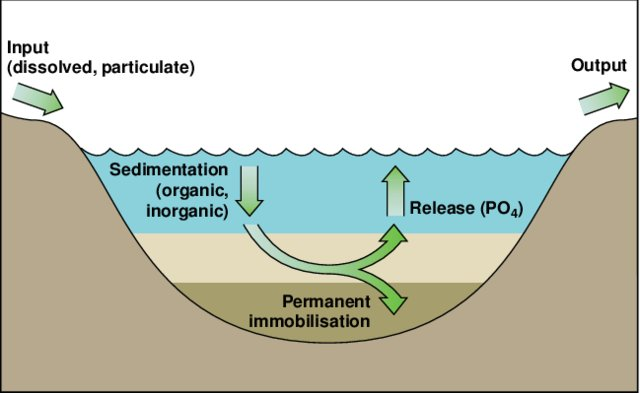
\includegraphics[width=0.75\linewidth]{C:/Users/harmv/Documents/studie/scriptie/Master/Master_Thesis/index/figures/load} 

}

\caption{Schematic illustrating the concept of internal P loading. P deposited in the lake sediment over time is released again.}\label{fig:intern}
\end{figure}
The increase of P levels from external sources such as wastewater or agricultural runoff is commonly referred to as the external P loading. From research on lake restoration during the 20th century it became clear that P released from sediment also plays a important role in P increase, and as the sediment can be regarded as part of the system, this release is defined as the internal P loading.\protect\hyperlink{ref-schindlerRecentAdvancesUnderstanding2006}{D. W. Schindler} (\protect\hyperlink{ref-schindlerRecentAdvancesUnderstanding2006}{2006}) When a freshwater system has experienced eutrophication from external sources over a long period of time, P is sequested in the sediment by OM deposition. (\protect\hyperlink{ref-oconnellChangesSedimentaryPhosphorus2020}{D. O'Connell et al. 2020}) The decomposing OM releases P to the water column, and this recycling of P can keep the water eutrophic for decades after external loading has been removed. (\protect\hyperlink{ref-chorusDecadesNeededEcosystem2020}{Chorus et al. 2020}; \protect\hyperlink{ref-sondergaardRetentionInternalLoading2001}{Søndergaard, Jensen, and Jeppesen 2001}) (Fig. \ref{fig:intern})

\hypertarget{measures-against-internal-p-loading}{%
\subsection{Measures against internal P loading}\label{measures-against-internal-p-loading}}

The extent of the ecological damage from eutrophication has lead to efforts to restore water quality of lakes and rivers in some places. However, eliminating external loading, by insulating the system from nutrient rich water sources in the vicinity and allowing only small-scale agriculture nearby, is often not sufficient, particularly if the system has been severely eutrophic for a long time. For P levels low enough to mitigate eutrophication and restore biodiversity, the internal P loading has to be lowered as well. Physical removing the sediment by dredging will remove some of the P rich layer, but is an expensive method and is not always effective as it is restricted in how much sediment can be removed, and high P concentrations often persist deep in the sediment. (\protect\hyperlink{ref-zamparasRestorationEutrophicFreshwater2014}{Zamparas and Zacharias 2014}) Moreover, it is an invasive technique which disturbs the sediment and risks contaminating the water. The problem of internal loading stems from the high dissolved fraction of P in the sediment, so a promising solution is to bind the P in the sediment so release is stopped. (\protect\hyperlink{ref-azamPhosphorousEnvironmentCharacteristics2019}{Azam et al. 2019}) Several materials have been mentioned to be used as a P adsorbtion agent to mitigate internal P loading, including modefied zeolites, lanthanum enhanced clays and alumininum compounds. (\protect\hyperlink{ref-azamPhosphorousEnvironmentCharacteristics2019}{Azam et al. 2019}) While some of the materials have a high adsorbtion capacity for P, a lot has to be added to effectively bind the large reservoir of P in the sediment, which can be an expensive endevour. Moreover, the solids could be buried deeper while phosphate rich sediment remains close to the surface, making this method less effective.

Iron (Fe) compounds are particularly of interest for P binding in the sediment. While less adsorbtive compared to materials designed to bind P such as lanthanum clays, iron is much cheaper and can easily applied in large quantities. Furthermore, the redox sensitivity of iron in the sediment can be an advantage, which was previously thought to lower its effectiveness as less adsorbtion sites become available. It has been shown that reductive dissolution mobilizing iron oxides as ferrous iron (Fe\(^{2+}\)) can recycle the iron by diffusion to the surface, where subsequent oxidation forms new iron oxides to bind P. (\protect\hyperlink{ref-kleebergHowEffectivelyDoes2012}{Kleeberg, Köhler, and Hupfer 2012}) This so called ``ferrous wheel'' forms in this way an effective trap for P leaving the sediment, and will remain in effect until the Fe pool is saturated with P. (Fig. \ref{fig:fwheel}) In addition, the Fe\(^{2+}\) and P can precipitate as vivianite (Fe\(_3\)(PO\(_4\))\(_2\))), removing the P from the system entirely. (\protect\hyperlink{ref-emersonEarlyDiagenesisAnaerobic1976}{Emerson 1976}; \protect\hyperlink{ref-rotheOccurrenceIdentificationEnvironmental2016}{Matthias Rothe, Kleeberg, and Hupfer 2016}) Fe can be added to the system in several forms: it can be dissolved in the surface water as salt, or directly as solid oxide. In this study we will focus on the effect of iron sludge from water treatment on internal P loading. Iron sludge is a byproduct consisting primarily of ferric (oxyhydr)oxides, and is available in large volume.
\begin{figure}

{\centering 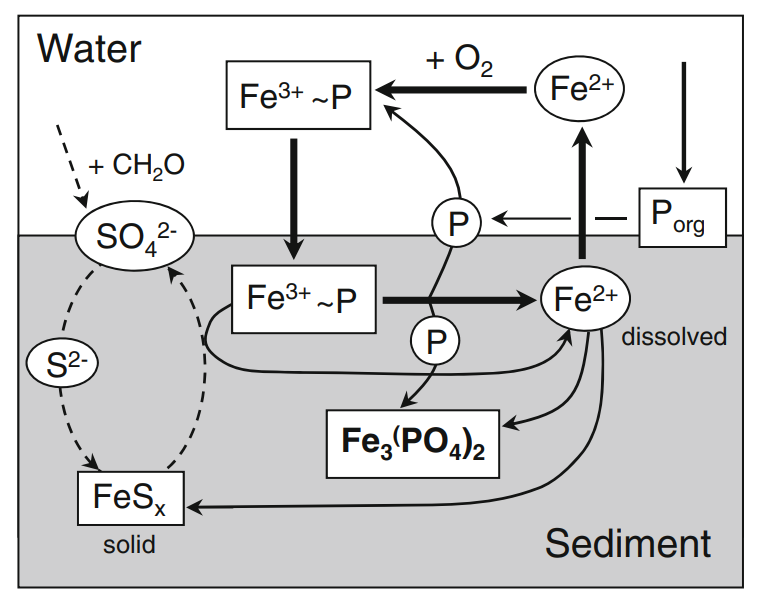
\includegraphics[width=0.8\linewidth]{C:/Users/harmv/Documents/studie/scriptie/Master/Master_Thesis/index/figures/ferrouswheel} 

}

\caption{Simple schematic representation of the ferrous wheel controlling the P dynamics in the sediment. Dissolved ferrous iron dffuses to the water column, where it is oxidized and precipititates together with phosphate. In the sediment it reduces and dissolves again, and thus forming a cycle. In this figure possibility of forming vivianite (Fe$_3$(PO$_4$)$_2$) is also presented. Fe is removed from the ferrous wheel when it reacts with dissolved sulfide, and precipitates. Figure modefied from  Kleeberg et al. (2012).}\label{fig:fwheel}
\end{figure}
\hypertarget{location-and-research-objective}{%
\subsection{Location and research objective}\label{location-and-research-objective}}

Treating freshwater systems with iron has been done before, and it has been shown that high sulfur (S) content can weaken the effectiveness by binding the iron as sulfide, which should be considered when calculating the necessary iron dose. \protect\hyperlink{ref-smoldersSulphatemediatedIronLimitation1993}{Smolders and Roelofs} (\protect\hyperlink{ref-smoldersSulphatemediatedIronLimitation1993}{1993}) Moreover, there have been indications that OM has strong interactions with both P and Fe. (\protect\hyperlink{ref-oconnellChangesSedimentaryPhosphorus2020}{D. O'Connell et al. 2020}; \protect\hyperlink{ref-schwertmannNatureIronOxide1988}{Schwertmann and Murad 1988}) It is therefore interesting to examine the application of iron addition to an environment rich in OM, such as peat lakes and ditches. \protect\hyperlink{ref-sondergaardRetentionInternalLoading2001}{Søndergaard, Jensen, and Jeppesen} (\protect\hyperlink{ref-sondergaardRetentionInternalLoading2001}{2001})

As part of the Rhine delta, marine clay deposition and peat layers formed the Western part of the Netherlands during the Holocene. Originally comprised of mainly inhabitable peat bogs and tidal marches, the area was drained and cultivated gradually during medieval times. A system of ditches, canals and lakes developed as a result of drainage practices, and the intensive extraction of peat as energy source. (\protect\hyperlink{ref-borgerDrainingDiggingDredging1992}{Borger 1992}) In an effort to stimulate dairy production, intense farming of cattle was introduced in the area during the 20th century. As a consequence, most surface water is highly increased in nutrients, and eutrophication is widespread. In recent years the negative effects of land reclamation and intensive agriculture of peat marches has attracted more attention. Dry peat soils cause subsidence and emit significant amounts of carbon dioxide. Efforts to re-wet parts of the western peat area are combined with restoration goals for biodiversity, as many meadow birds characteristic for this kind of landscape can thrive on wet grassland. However, the plentiful lakes and ditches in the area remain polluted by nutrients. (\protect\hyperlink{ref-keizerPhosphorusSedimentLoosdrecht1992}{Keizer and Sinke 1992}) Improvement of surface water quality is essential to restore the nutrient poor conditions of biodiverse types farmland common in this area before the industrial revolution.

In this study, we investigate the realized treatment of a peat extraction ditch with iron sludge. If iron treatment is to be used in similar places again, a thorough understanding of the processes in the sediment are desired. By analyzing samples from the field in detail and monitoring the nutrient dynamics under laboratory conditions, we aim to answer the following questions:
\begin{itemize}
\item
  Can the treatment iron be recognised in the sediment, and what is the iron speciation?
\item
  Did iron treatment bind P in the sediment, in which binding form?
\item
  How does iron treatment influence the internal P load in peat extraction ditches?
\end{itemize}
\hypertarget{methodology}{%
\section{Methodology}\label{methodology}}

\hypertarget{study-site}{%
\subsection{Study site}\label{study-site}}

Sediment cores and surface water were gathered at Bovenlanden, a peat meadow in South-Holland, the Netherlands. (Fig. \ref{fig:BL}) The area functioned as farmland in the past, and is heavily influenced by fertilization. Nowdays, Bovenlanden is managed by Natuurmonumenten, in a conservation effort to restore biodiversity in the western peat meadow system of the Netherlands. The goal is to restore types of grassland common before industrialization of farming, which have typically more diverse vegetation and form a habitat for breeding meadow birds. To establish a nutrient poor wet meadow, an effort was needed to improve water quality. To reduce external nutrient load, most ditches in the southern part have been detached from the surrounding surface water, keeping only one inlet via a weir, and runoff from land was reduced by removing the top layer of soil containing most of the nutrients. In 2020, 60 tons of iron sludge was added to the southern two ditches to mitigate internal P loading. Water quality improved on visual inspection after a few months after the treatment.
\begin{figure}

{\centering \includegraphics[width=1\linewidth]{C:/Users/harmv/Documents/studie/scriptie/Master/Master_Thesis/index/figures/BovenlandenOverview} 

}

\caption{Overview of the study site. On the left  the general location within the Netherlands is shown. In the bottom right is indicated where Bovenlanden is located within the Western peat area. On the right a satelite image of Bovenlanden with important features highlighted. Two ditches in the area have been treated with iron sludge in the past. Note the only water inlet is located in the north, far away from the treated ditches}\label{fig:BL}
\end{figure}
\hypertarget{core-sampling}{%
\subsection{Core sampling}\label{core-sampling}}

The site was visited the 23rd of February 2021 to collect sediment cores. Two locations on the same treated ditch were chosen based on distance from the inlet weir, each treated location was paired with a reference location in a non-treated ditch nearby. (Fig. \ref{fig:sampleloc}) For each of the four locations 7 cores were collected using a UWITEC corer with a diameter of 6 cm. Sediment depth in the cores was approximately 40 cm, with 20cm overlying water. Extra surface water was collected for refilling during incubation sampling. Temperature, PH, dissolved oxygen, and electrical conductivity were measured using probes. Surface water samples where collected and filtered on site using 0.45\(\mu\)m pore size syringe filters.
\begin{figure}

{\centering \includegraphics[width=1\linewidth]{C:/Users/harmv/Documents/studie/scriptie/Master/Master_Thesis/index/figures/BovenlandenSampleLocations} 

}

\caption{Four location within the Bovenlanden system where samples have been taken. On the northern of the two treated ditches, two locations on opposide sides were chosen: A and C. To differentiate from the non-treated locations, they are displayed in red. Two nearby locations in untreated ditches, B and D, are displayed in blue. The two sides of the ditch were chosen to investigate the possible influence of surface water influx, as locations B and D are closer to the water inlet in the north of the system. }\label{fig:sampleloc}
\end{figure}
Directly after the field campaign, one core from each location was sliced for porewater and sediment analysis. Slicing was performed under low oxygen conditions in intervals of 1cm for the top 10cm, and 2cm intervals at greater depth. Sediment slices were collected in 50mL centrifuge tubes and centrifuged at 3000rpm for 10min to seperate porewater. In a glovebox with nitrogen atmosphere, the porewater was decanted into a syringe with a 0.45\(\mu\)m filter and filtered into subsamples. The sediment was freezedried, and homogenized with an agate mortal and pestle under nitrogen atmosphere. Wet samples were stored cool (5°C) in airtight containers, dry sediment was kept under nitrogen atmosphere.

\hypertarget{sequential-extractions-of-fe-pools}{%
\subsection{Sequential extractions of Fe pools}\label{sequential-extractions-of-fe-pools}}

Analysis of the iron pools in the solid phase was done with a sequential extraction method based on \protect\hyperlink{ref-claffSequentialExtractionProcedure2010}{Claff et al.} (\protect\hyperlink{ref-claffSequentialExtractionProcedure2010}{2010}). The method was modified to include phosphate measurements of the extracted pools by omitting the pyrophosphate extraction in the main sequential extraction. Parallel to the main extraction a two-step extraction of MgCl and pyrophosphate was performed to target the organic bound iron. (Table \ref{tab:seqextr})

Approximately 100mg of dry sediment was weighed into a 15mL centrifuge tube. For each extraction step, 10 mL of extraction solution was added with a dispenser under a continue nitrogen flow. After addition, the mixture was weighed, resuspended and shaken for a specified time. After extraction, the suspension was centrifuged for 10min at 3000rpm, and the supernatant decanted into a syringe with 0.45\(\mu\)m filter and the next extraction solution was added immediately. The extractant was filtered and diluted 10 times before analysis. The last extraction step, which uses concentrated nitric acid, was not filtered but diluted 100 times.
\begin{table}[ht]
 \centering
     {\footnotesize
        \begin{tabular}{m{0.1\textwidth} m{0.07\textwidth} | m{0.1\textwidth} m{0.3\textwidth} m{0.1\textwidth} m{0.2\textwidth}}
            \hline \hline
                  & step  & name & extractant & extraction time & target pool      \\
            \hline
                Extraction A   & 1 & MgCl & 1M magnesium chloride solution & 1h & exchangable iron, iron salts \\
                   & 2 & HCl & 1M hydochloric acid & 4h & easily dissoluble iron oxides and sulphides, carbonates\\
                   & 3 & CBD & 50 g/l sodium dithionite in 0.35 M acetic acid and 0.2 M sodium citrate buffer (pH 4.8)  & 4h & crystalline iron oxides \\
                   & 4 & HNO$_3$ & concentrated nitric acid (67\%)& 2h & pyrite\\
                   \hline
                    Extraction B   & 1 & MgCl & 1M magnesium chloride solution & 1h & exchangable iron, iron salts\\
                    & 2 & pyrophosphate & 0.1M sodium pyrophosphate solution & 16h & organic bound iron\\
            \hline \hline
        \end{tabular}}
    \caption{Sequential extraction procedure for determining Fe speciation. The extraction is performed in multiple steps using different solvents to extract iron phases. The sequence is build up so each step targets a subsequent pool with lower reactivity. The procedure is modefied from @claffSequentialExtractionProcedure2010 by removing the organic targeting pyrophosphate extraction from the sequence and instead to perform a parallel pyrophosphate extraction, here listed as extraction B.  }
    \label{tab:seqextr}
    \end{table}
\hypertarget{incubation-setup-for-benthic-flux-measurements}{%
\subsection{Incubation setup for benthic flux measurements}\label{incubation-setup-for-benthic-flux-measurements}}

To monitor benthic fluxes under oxic and anoxic conditions, sediment cores where incubated in a climate chamber at 10°C for 60 days. For each location two cores were allowed to turn anoxic, and two where kept oxic by aerated the overlying water. To induce anoxic conditions, the cores were closed with an airtight cap with a stirrer and filled completely with surface water. (Fig. \ref{fig:setup}) The decay in oxygen was monitored with an oxygen probe. Change in concentration of the overlying water was monitored by taking 20 mL from 1-3 cm above the sediment-water interface using a syringe and rubber tube, and filtered through a 0.45\(\mu\)m syringe filter directly into subsamples. The water was replenished using surface water collected at the locations, in the anoxic cores this was done simultaneously when taking samples to prevent air entering the core. Samples where taken from the overlying water on daily basis the first two weeks, and 2-3 times a week for the remaining experiment. At the end of the experiment, one anoxic core for each location was sliced and processed for porewater and sediment analysis.
\begin{figure}

{\centering 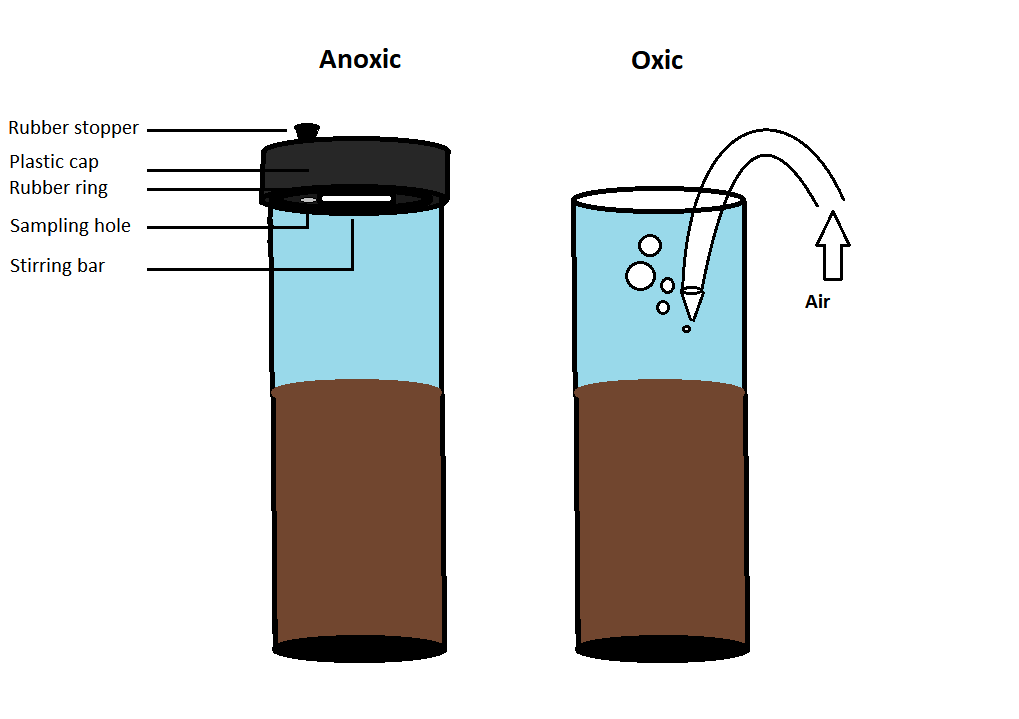
\includegraphics[width=0.4\linewidth]{C:/Users/harmv/Documents/studie/scriptie/Master/Master_Thesis/index/figures/Schematic} 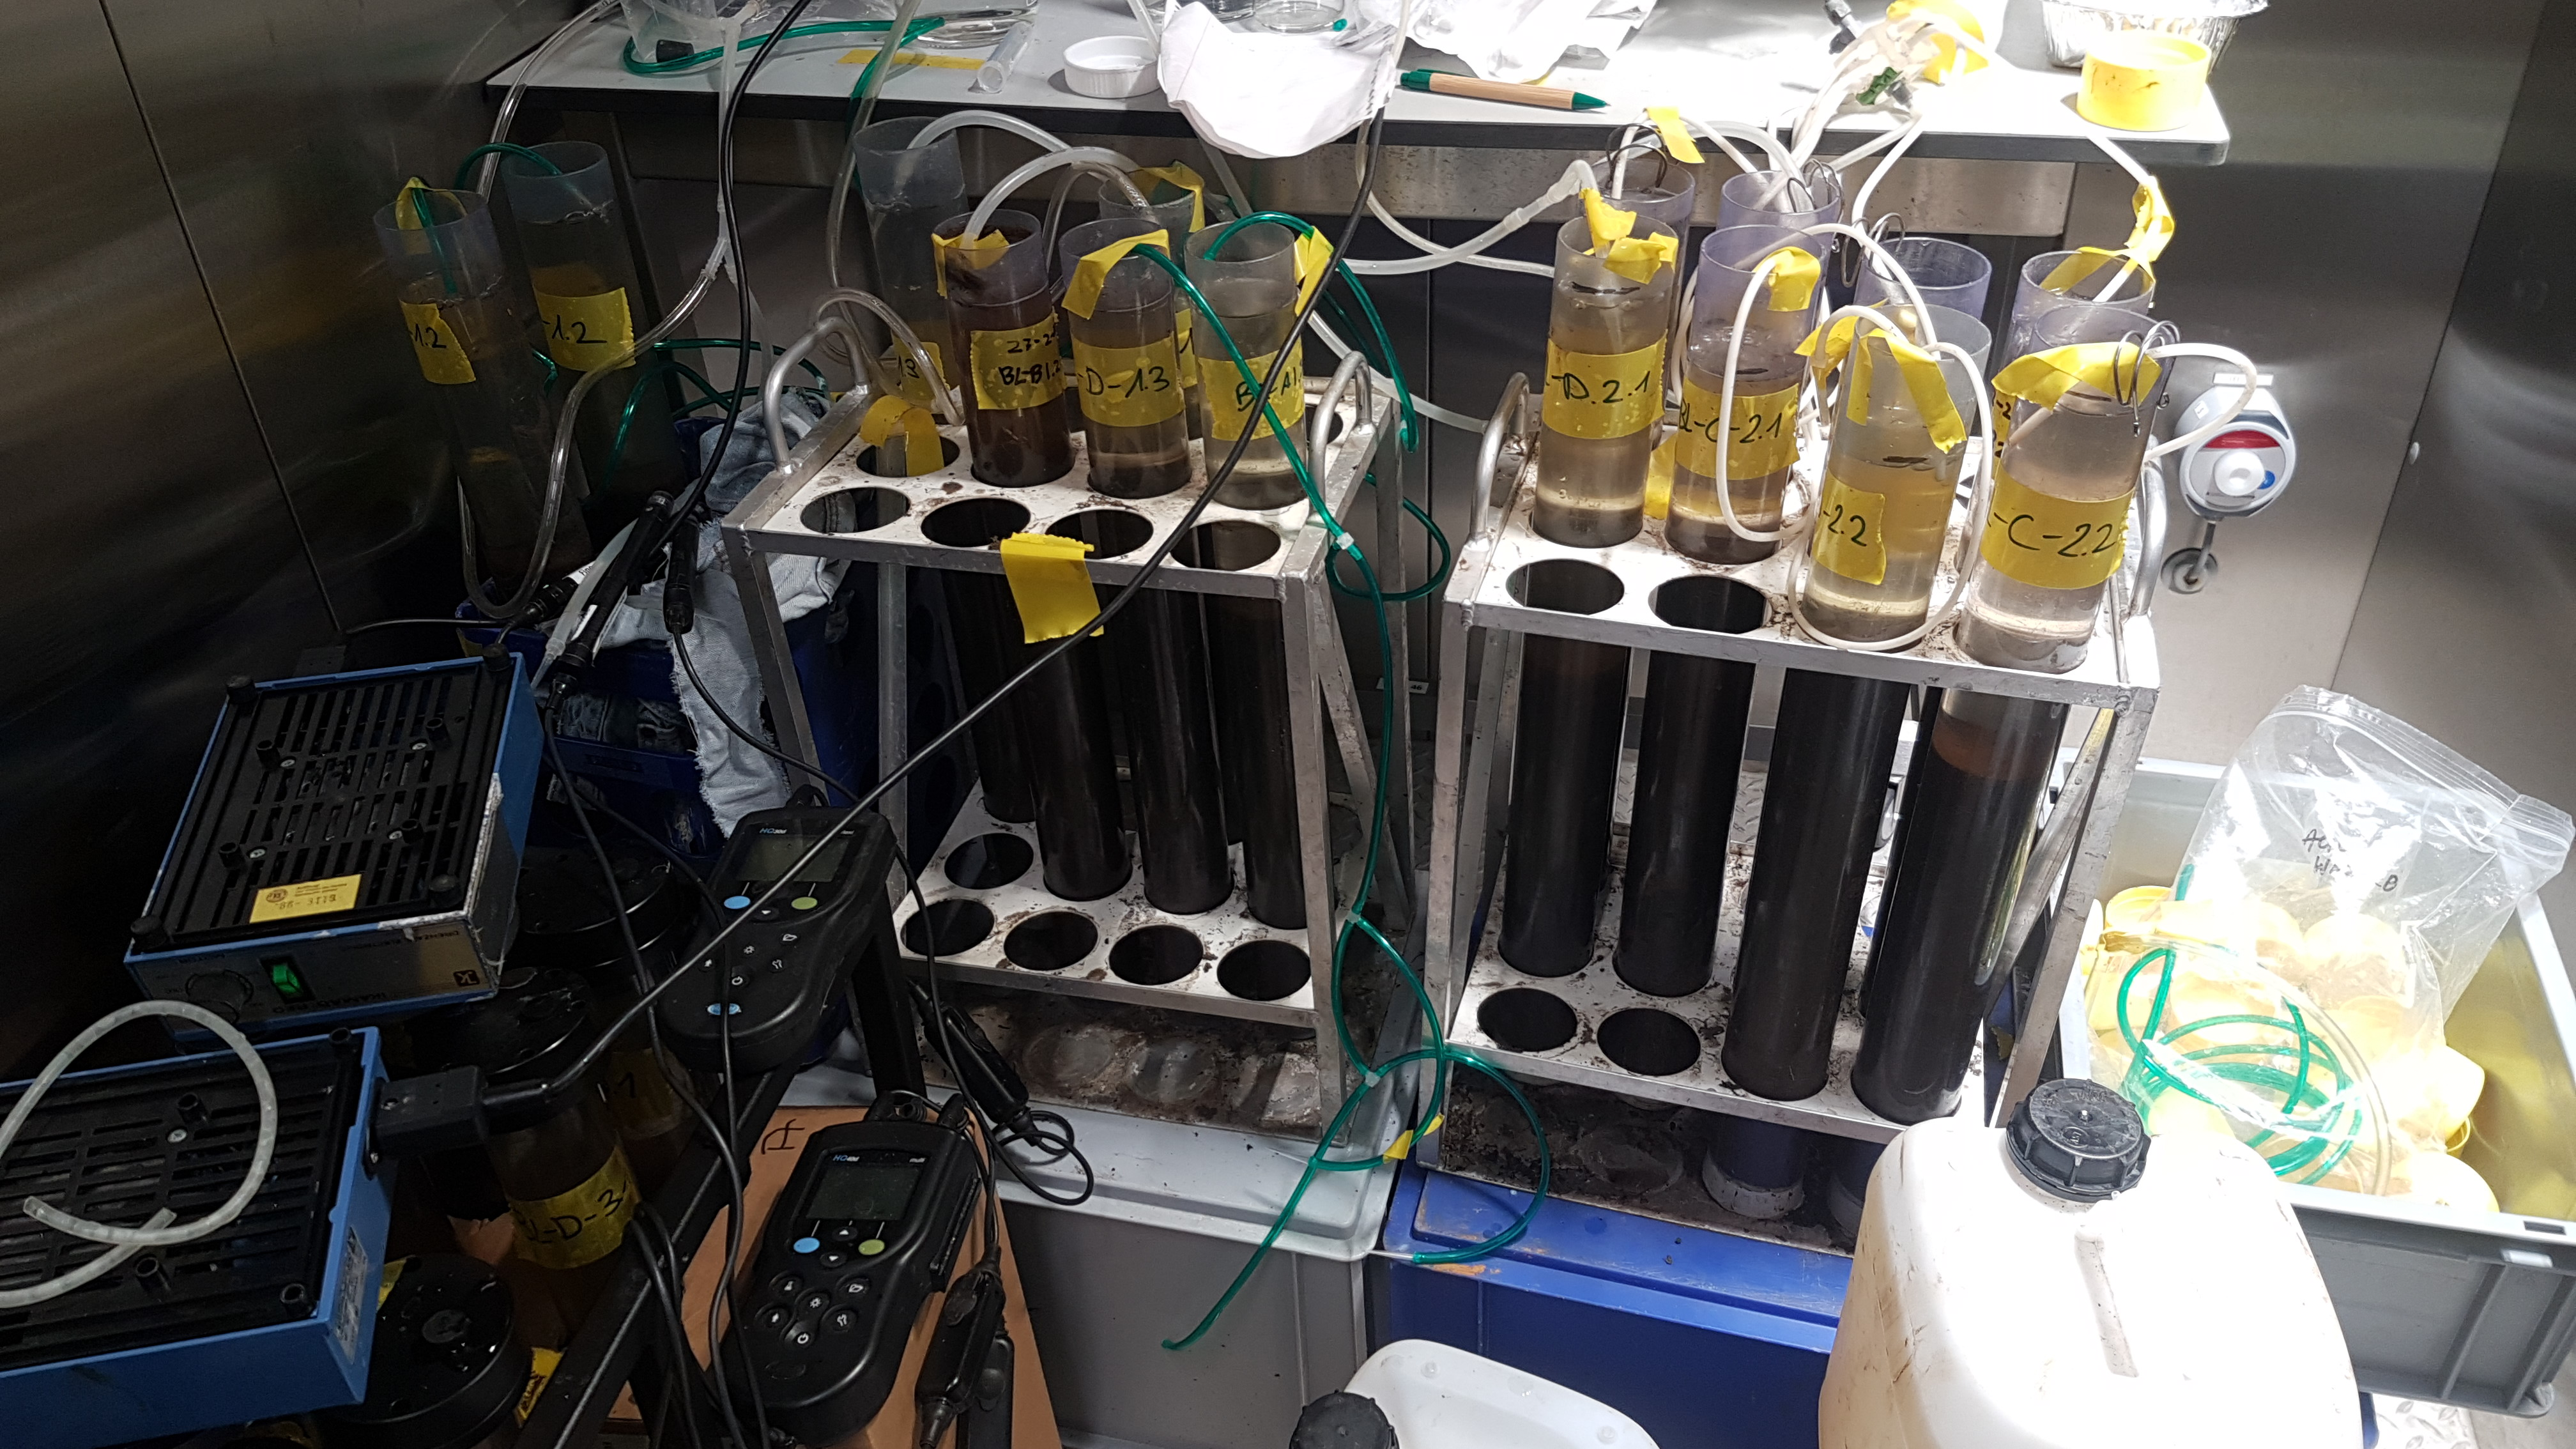
\includegraphics[width=0.4\linewidth]{C:/Users/harmv/Documents/studie/scriptie/Master/Master_Thesis/index/figures/setup} 

}

\caption{Incubating cores to monitor benthic fluxes. Left: Schematic representation of the anoxic and oxic incubations. Right: Photograph of the climate chamber during the experiment. In the center the oxic cores are aerated through tubes, while in the down-left corner the anoxic cores are contnuously stirred by upside-down magnetic stirrers.}\label{fig:setup}
\end{figure}
\hypertarget{quantification-methods}{%
\subsection{Quantification methods}\label{quantification-methods}}

Surface water, incubation samples and porewater were analyzed on phosphate, total iron, ferrous iron (Fe\(^{2+}\)), sulfide and ammonium with spectrophotometry following standardized methods using coloring reagents.(\protect\hyperlink{ref-murphyModifiedSingleSolution1962}{Murphy and Riley 1962}) For P and Fe measurments, a subsample was acidified after sampling with 1\% 3.75M HNO\(_3\) to prevent oxidation. (\protect\hyperlink{ref-brayPhosphateInterstitialWaters1973}{Bray, Bricker, and Troup 1973}) Calibration lines for ammonium, total iron and Fe\(^{2+}\) were freshly made every day of measurement, while the phosphate calibration line was made once and remeasured. For calibrating sulfide measurements, a calibration slope of a previous experiment was used. Water samples were also measured by ion chromatography (IC), to quantify common anions including sulfate and nitrate. The IC reported phosphate concentrations as well, but were not used since the reported values of P were higher than determined with spectrophotometry, and with much larger variability. The diluted extraction solutions gathered during the sequential extraction procedure were analyzed by inductively coupled plasma optical emission spectrometry (ICP-OES). In addition, spectrophotometry was deployed to identify the oxidation state of dissolved iron, which was only possible in the HCl extracted pool, as CBD and concentrated HNO\(_3\) strongly influence the redox potential, and the MgCl and pyrophosphate pools were exposed to oxygen during the extraction procedure. The low pH of HCl stabilizes the redox state, and since it extracts various different reactive iron species, an evaluation on the redox state is useful. However, many values of Fe\(^{2+}\) were found higher than total iron concentration. Total iron measured with spectrophotometry correlated strongly with ICP-OES Fe data, and is thus considered to be more reliable than the Fe\(^{2+}\) results, which are excluded from this study.

\hypertarget{results}{%
\section{Results}\label{results}}

The \textit{in situ} surface water measurements showed that both at the treated and non treated locations oxic conditions of 9.5-10.5 mg/L dissolved oxygen, and pH levels around 8. While no significant difference between treated and non-treated locations, water conditions did vary between the locations closer (C and D) and further away (A and B) from the water inlet. This variation was seen in a significantly higher electric conductivity at locations A and B (438 \(\mu\)S and 451\(\mu\)S), than measured at locations C and D (395\(\mu\)S and 397\(\mu\)S), which correlated with sulfate concentrations. In addition, the decrease in sulfate concentration with depth in the porewater was steeper in locations C and D compared to A and B.( Fig. \ref{fig:pwprofiles})

Differences in iron content are immediately clear when comparing the sequential extraction data, which shows that iron is much more abundant in the treated cores than in the non-treated.(Fig. \ref{fig:seq}, left panel) The largest pool extracted in the treated sediment is the HCl extractable pool, while the orginal sediment contains predominantly iron extracted HNO\(_3\). The small amount of other Fe extracted in the non-treated cores is restricted to the top few centimeter. Interestingly, the HNO\(_3\) extracted Fe after treatment is lower than in the original sediment.
\begin{figure}

{\centering 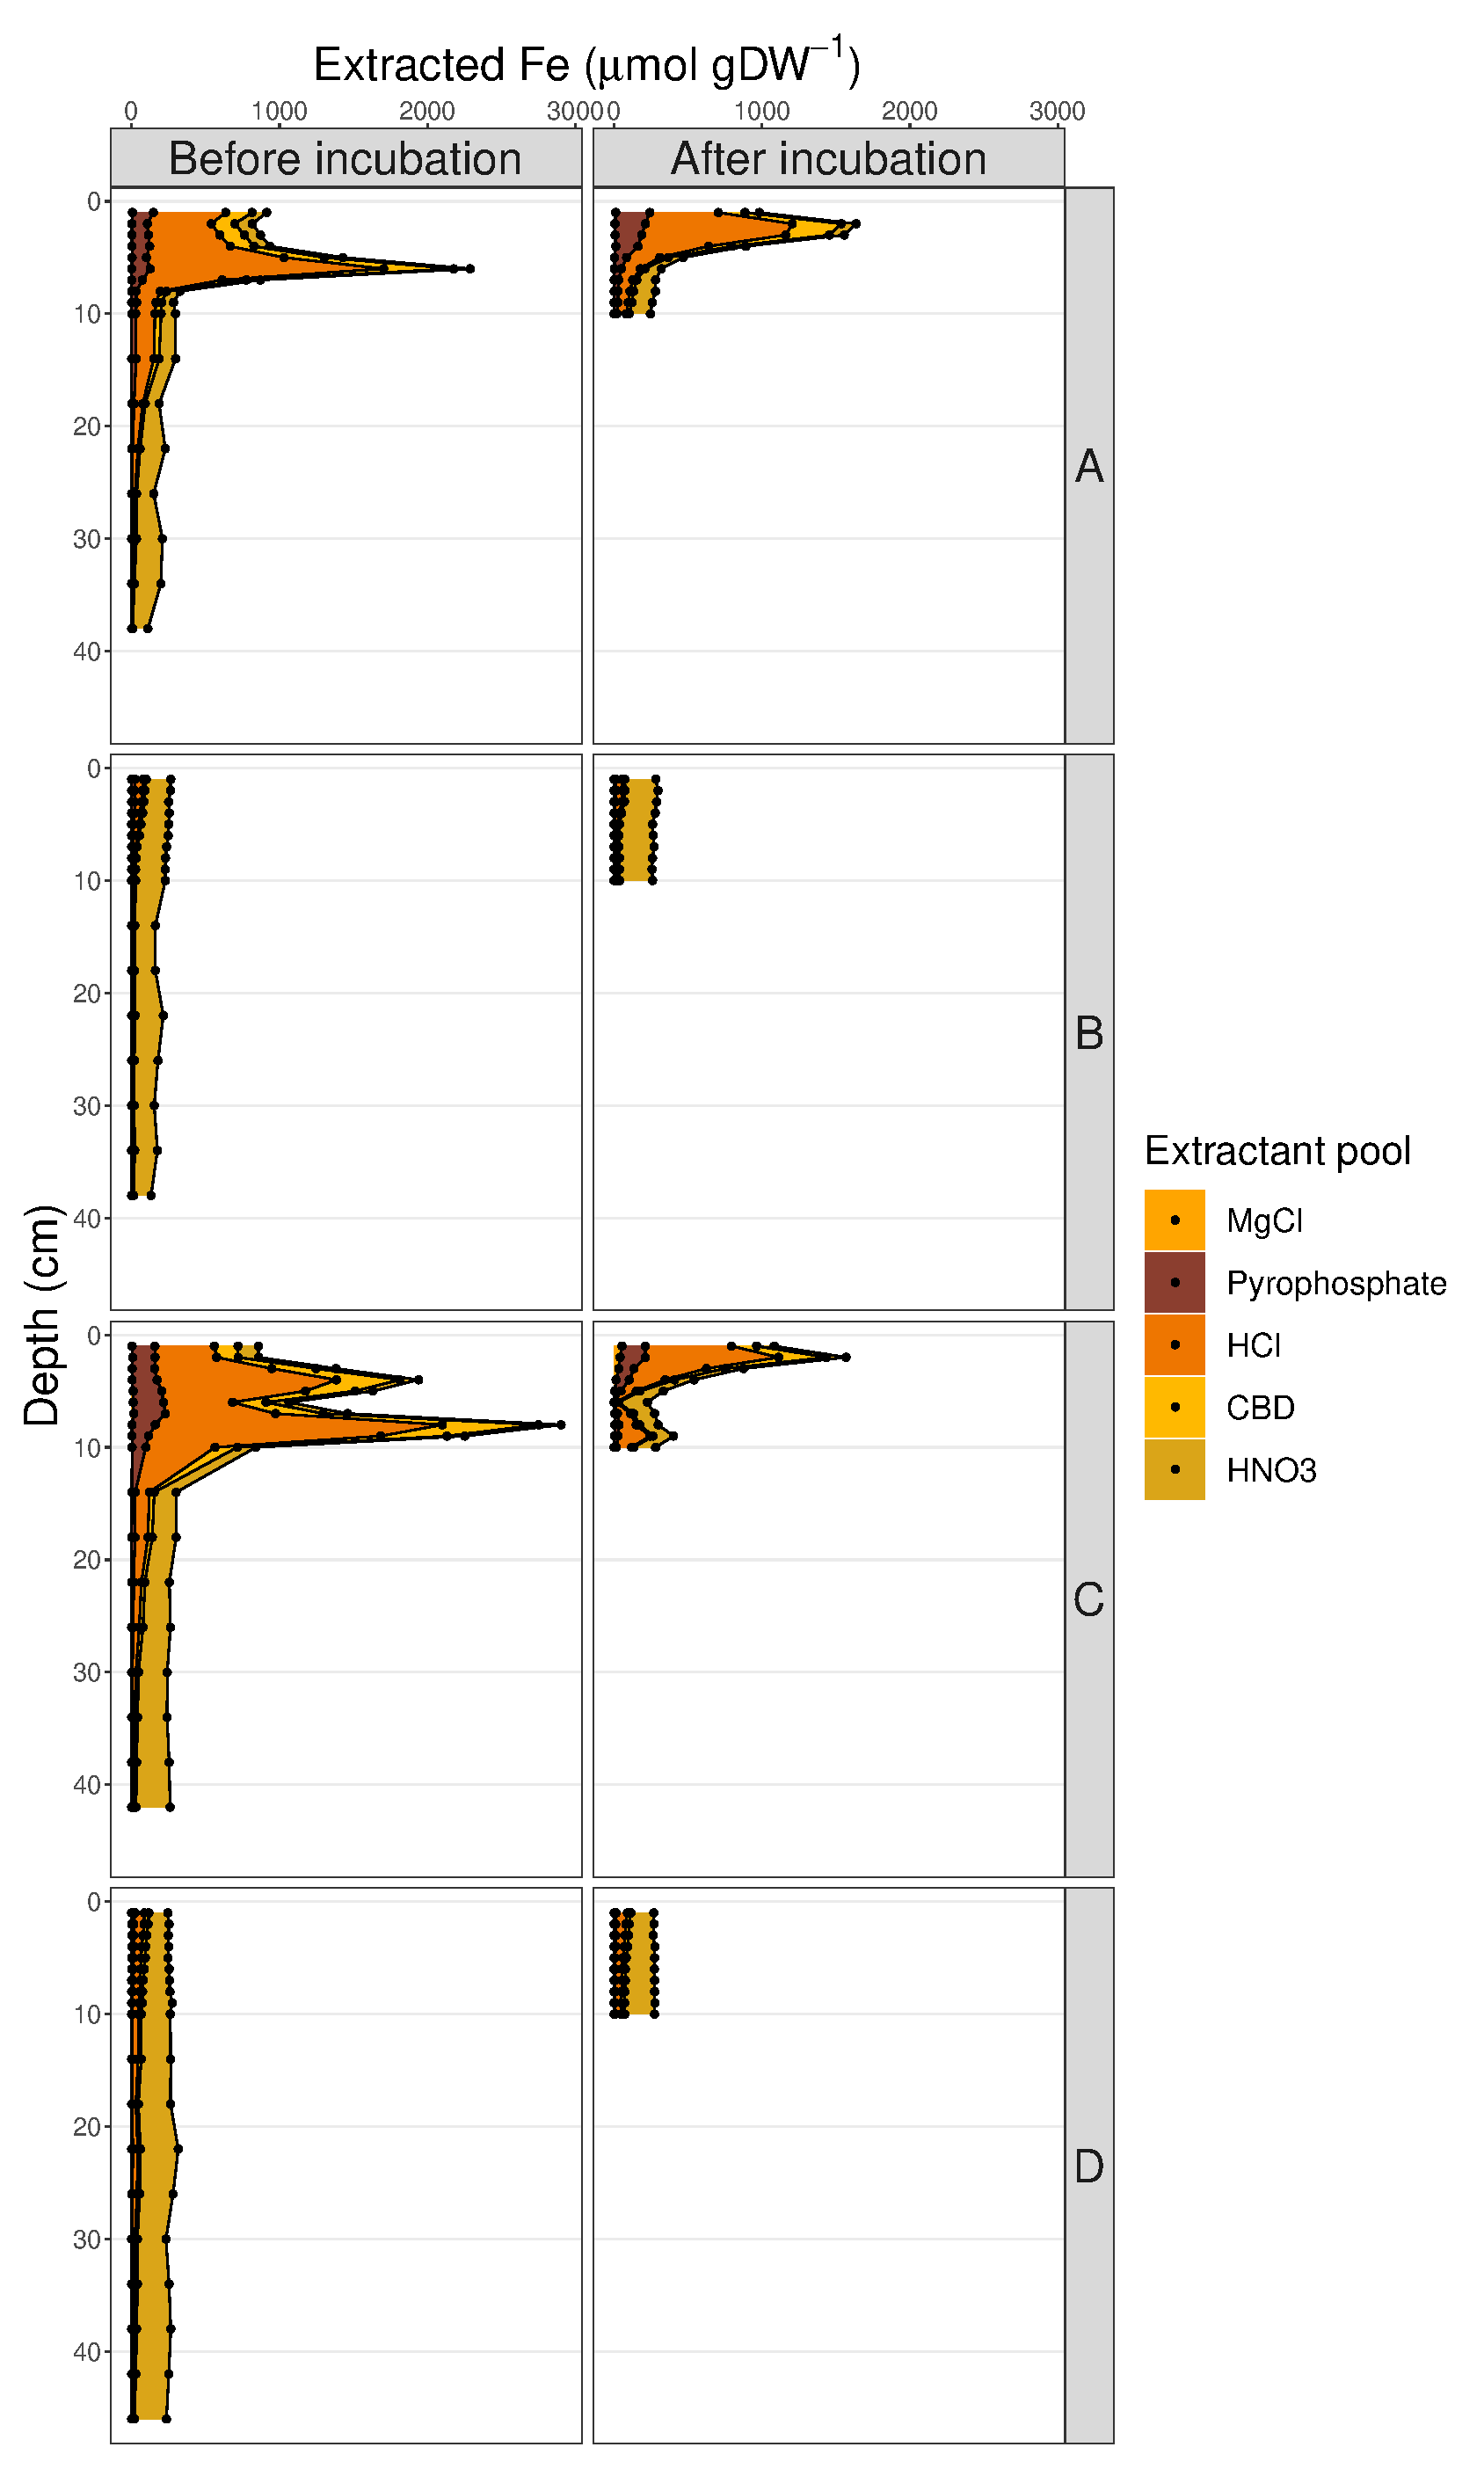
\includegraphics[width=0.45\linewidth]{C:/Users/harmv/Documents/studie/scriptie/Master/Master_Thesis/index/figures/seq_extr_Fe_2} 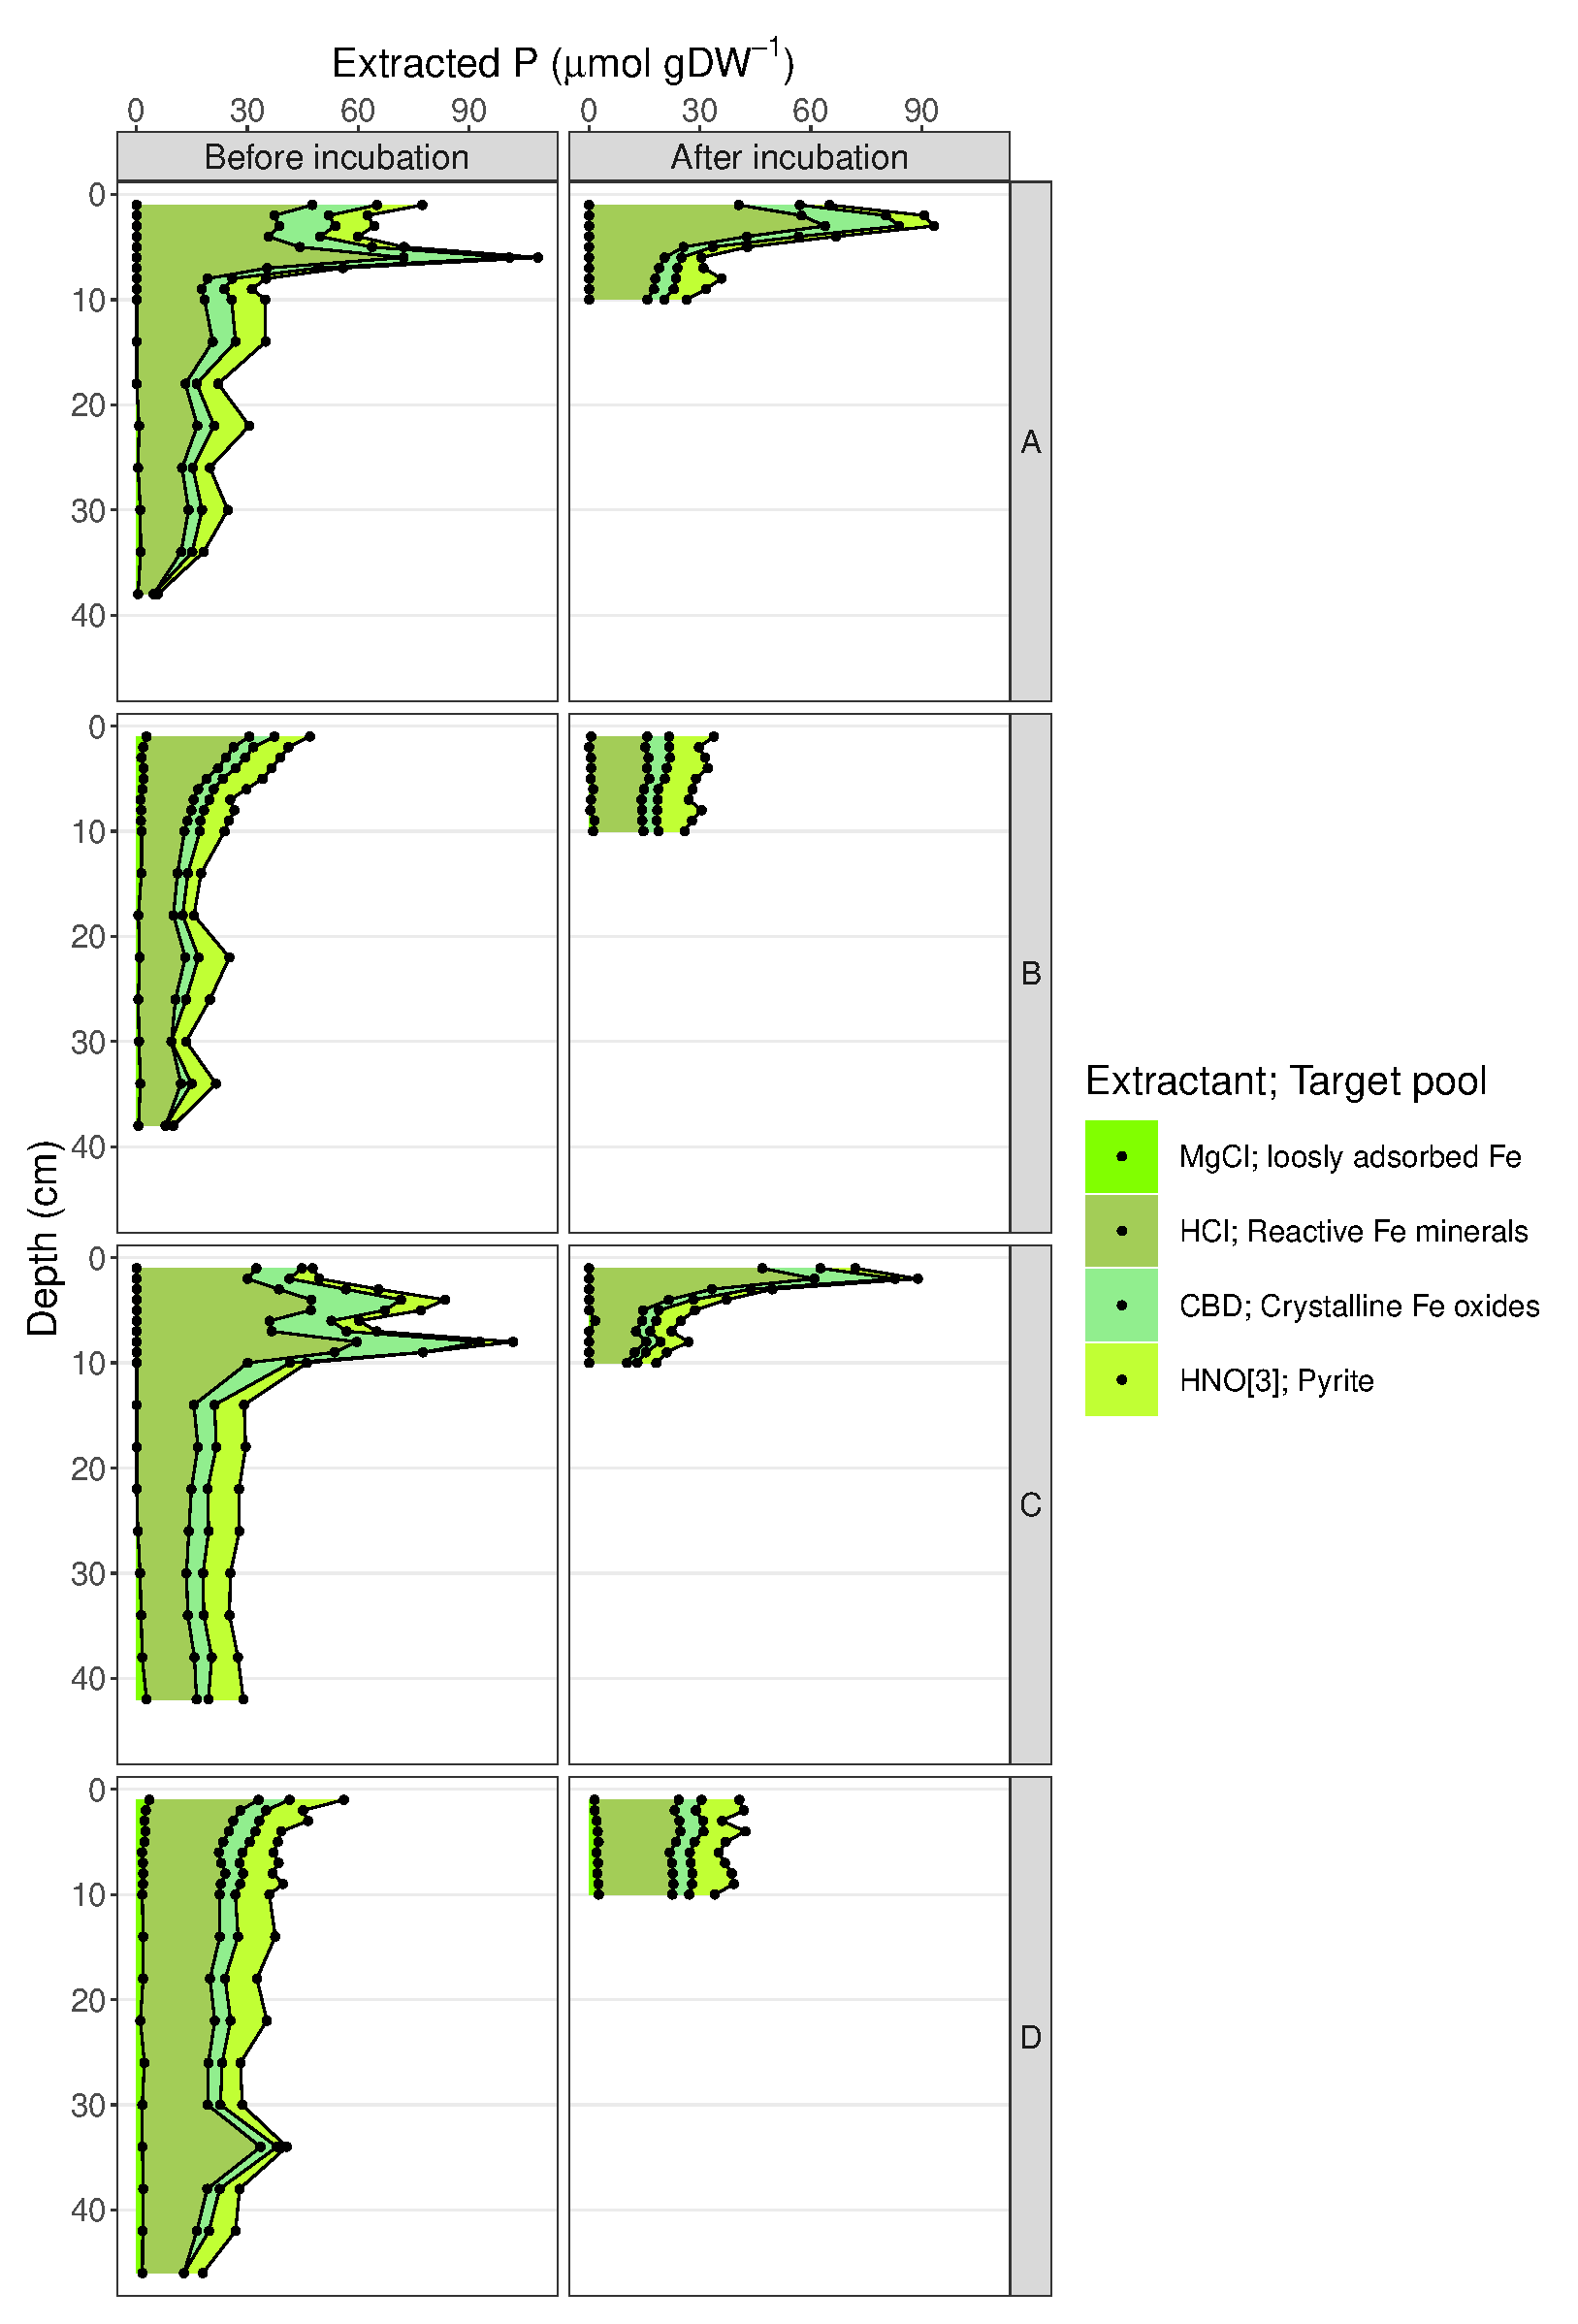
\includegraphics[width=0.45\linewidth]{C:/Users/harmv/Documents/studie/scriptie/Master/Master_Thesis/index/figures/seq_extr_Fe_3} 

}

\caption{Diagram outlining the sequential extraction results. The extracted Fe and P for each extraction step is plotted as function of depth. Left panel shows the extracted Fe in each pool, the right panel the P.  The stacked and coloured integrals represent the relative size of the corresponding extacted pool and the total width the sum of all pools. The pyrophosphate extraction was performed in parallel, and is subsracted from the HCl pool in the Fe data. P was not analyzed in the pyrophosphate pool, it is assumed the pyrohosphate extractable P is distributed over the other pool.    }\label{fig:seq}
\end{figure}
In addition to sediment from cores which were sliced and processed directly after the field campain, some cores used in the benthic flux experiment were sliced after the experiment ended, to evauate the effect of anoxic water conditions on the sediment. Significantly more Fe was extracted with HNO\(_3\) from non-treated cores analyzed after anoxic incubation than found in fresh cores. In contrast, the rest of the extracted pools, in particular the HCl pool, decreased in iron content. Becouse of meso-scale heterogeneity of horizontal iron sludge distribution in the treated ditch, the Fe content varies greatly between cores, and absolute size of the pools can therefore not be compared. However, since the iron speciation in the sludge is the same in every location, the relative changes of Fe pools can be used to inspect changes between cores before and after incubation. To only compare changes in the treated Fe, the Fe content of the reactive pools relative to the CBD pool was taken, with the assumption that the CBD pool mainly comprises stable iron oxides which have not changed significantly. Here, a relative increase in both the pyrophosphate and HCl extracted iron pools is striking. The variation in iron content also explains the difference in vertical Fe distribution between cores, as larger clumps of iron sludge sink deeper in the sediment.

Phosphate in the extracted pools correlates with the Fe distribution in the HCl pool. While HCl extracted Fe is only a small fraction in the non-treated cores, the extracted P is largest in this pool. (Fig. \ref{fig:seq}, right panel) The treated sediment extracted more P with HCl at the maxima of iron, but was not that much higher compared to P in the untreated sediment. This leads to much higher P/Fe ratios in the HCl pool of the non-treated than the treated cores, respectively finding average P/Fe ratios of \(0.358\pm 0.058\) and \(0.052 \pm 0.013\) within 10cm depth.
\begin{figure}

{\centering \includegraphics[width=1\linewidth]{C:/Users/harmv/Documents/studie/scriptie/Master/Master_Thesis/index/figures/profiles} 

}

\caption{Depth profile of nutrient concentration in porewater. Treated locations are shown in red, non-treated reference locations in blue. Top row shows cores sliced directly after sampling, the bottom row after two months incubating under anoxic conditions. Iron, phosphate, slufide and ammonia were measured with photospectometry, sulfate and nitrate with IC.}\label{fig:pwprofiles}
\end{figure}
In line with the change in solid phase composition, the porewater content also differs between treated and non-treated locations.(Fig. \ref{fig:pwprofiles}) Treated cores contain high concentrations of iron in both oxidation states at depths with high solid iron content, with Fe\(^{3+}\)/Fe\(^{2+}\) exceeding 1, meaning much of the iron is found in oxidized form. Dissolved iron is highest at 1 - 10 cm depth in treated cores, and below the zone where solid iron is concentrated it is mainly reduced Fe\(^{2+}\) and decreases with depth. In contrast, porewater of the non-treated cores contain very little iron. For phosphate an opposite trend can be seen: The non treated cores have high concentrations of phosphate in their porewater at every depth, with a peak in concentration close to the surface and an increase with after \textasciitilde10 cm. Phosphate concentrations in the porewater, however, are low (\textasciitilde1-10 \(\mu\)M) where the dissolved iron concentration is high, and increase only with depth after 10 cm. A similar, stronger effect is seen in the sulfide distribution, where high porewater concentrations found in the untreated sediment are absent in the presence of dissolved iron.
\begin{figure}

{\centering 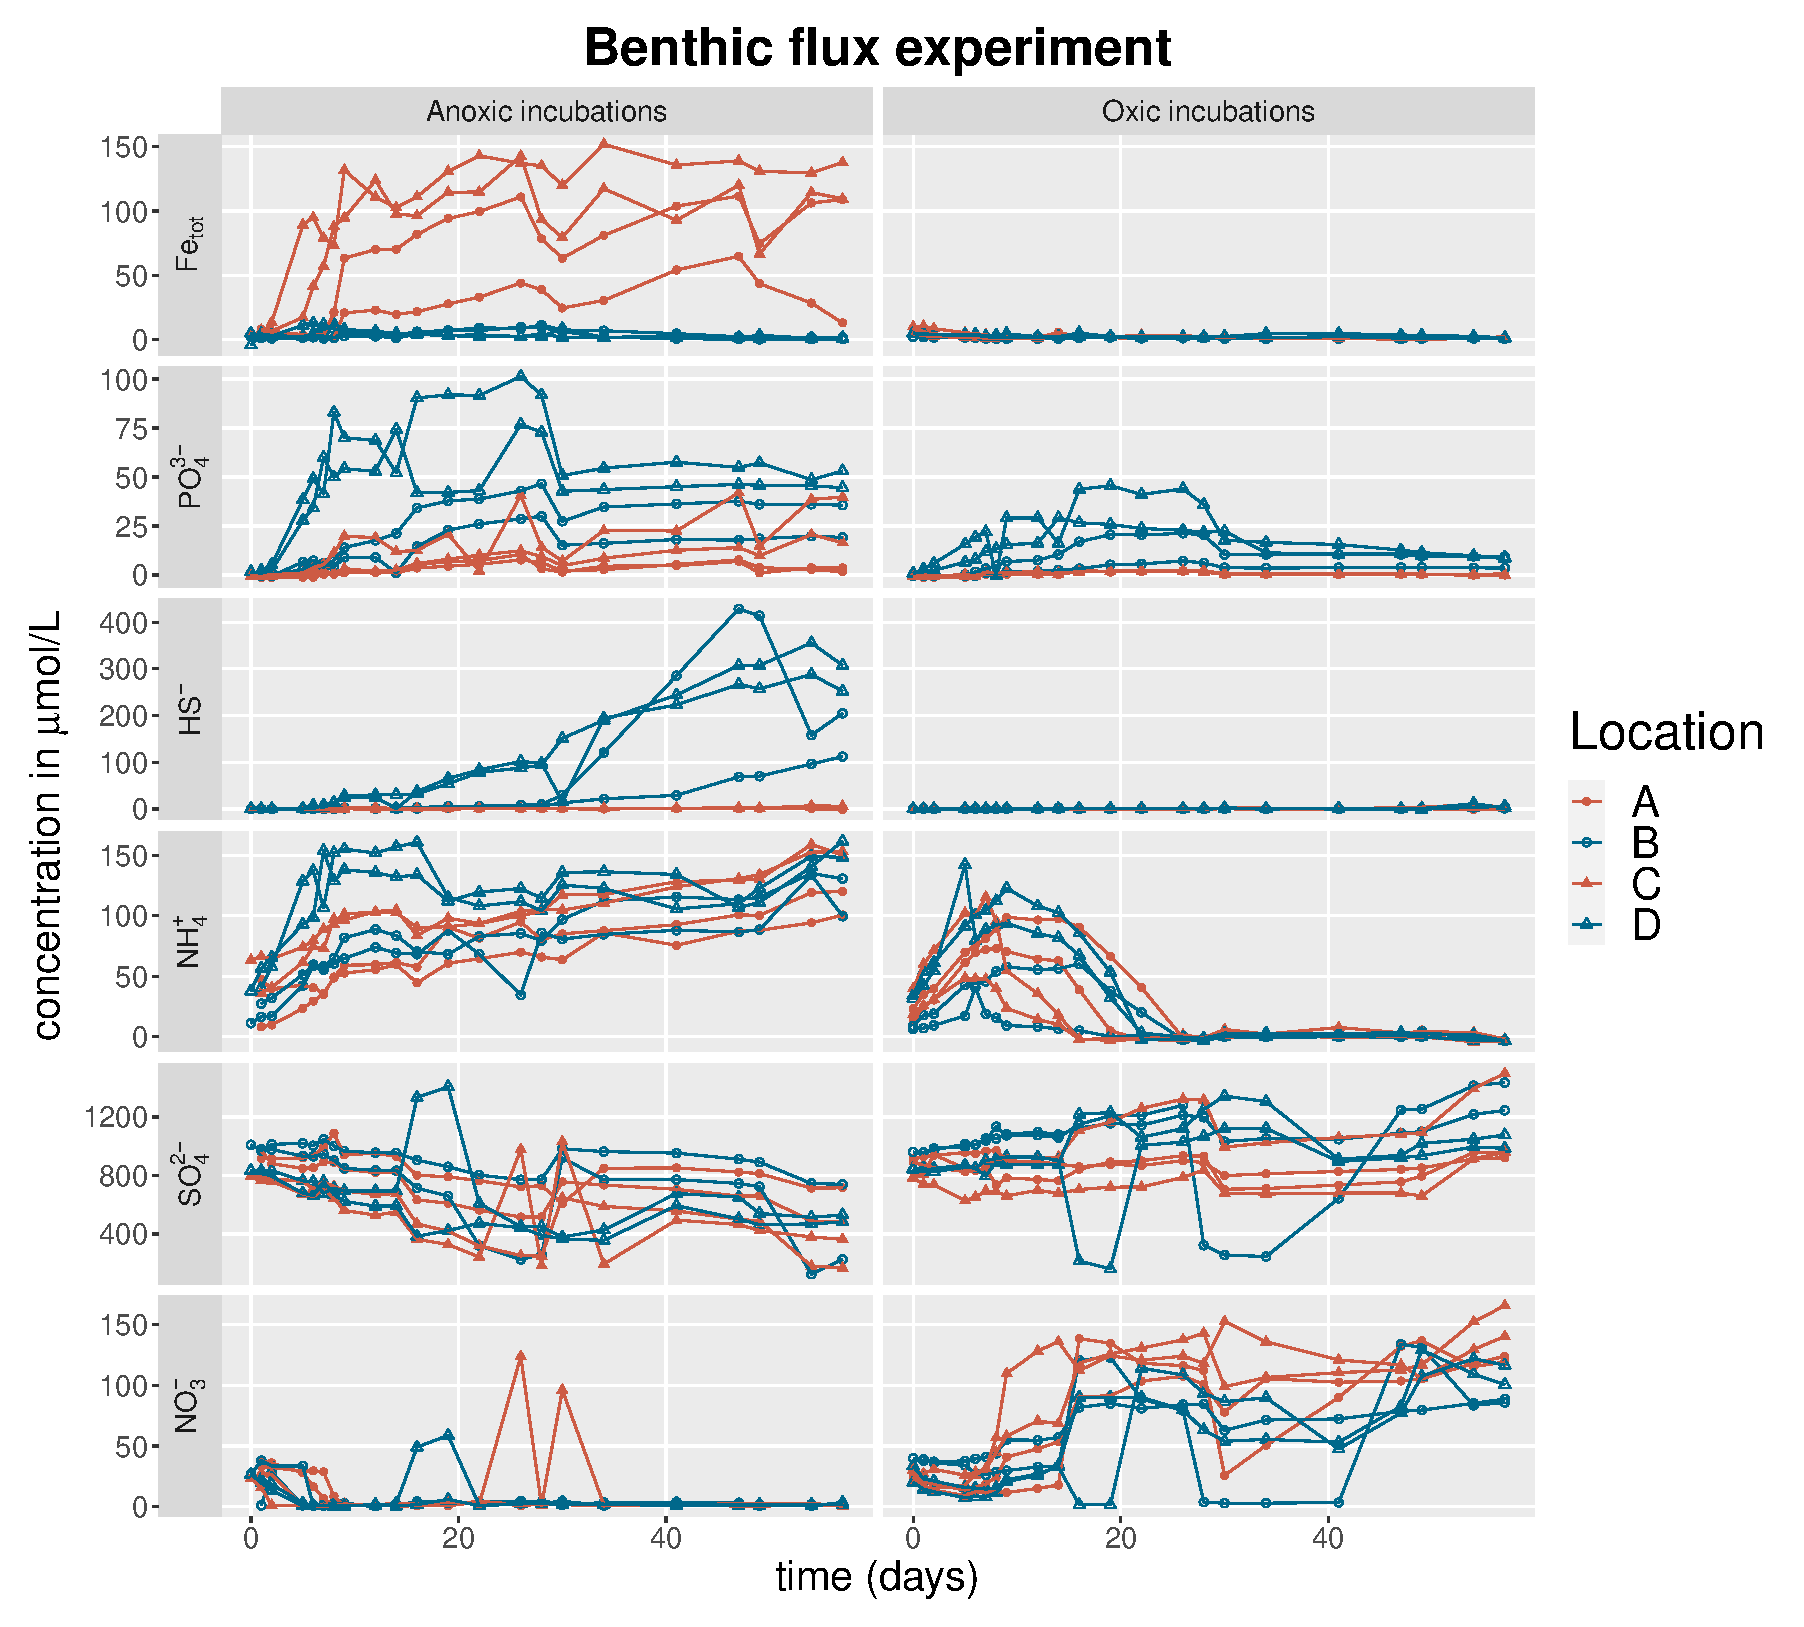
\includegraphics[width=0.85\linewidth]{C:/Users/harmv/Documents/studie/scriptie/Master/Master_Thesis/index/figures/IC_incubations_1} 

}

\caption{Concentration of nutrients in overlying water of incubated cores over time. Cores with anoxic conditions induced during the experiment (*left colum*) are compared with cores kept oxic by continue aeration (*right column*). The main goal was to study the difference in benthic fluxes from treated sediment, here in red, in relation to untreated sediment, displayed in blue. There are two treated and two untreated locations,  every location is incubated in duplo. The scale of the y axis is different for each parameter, while the x axis representing time in days is the same for all.}\label{fig:incubations}
\end{figure}
The benthic flux experiment shows the release of nutrients over time, and indicates changes the benthic fluxes of Fe, P and S in particular as effect of Fe treatment.(Fig. \ref{fig:incubations}) P concentrations are largest in non-treated cores, and remain much lower in surface water of treated cores. There is a clear coupling between P release and redox conditions, which is stronger in the treated cores. Fe increase is almost completely dependent on redox conditions, and is exclusively seen in the anoxic cores. The iron increase is characterized by a sharp increase at the start of the experiment, which halts after a while. In the treated cores this increase leads to fluxes of iron in the order of 1-3mmolm\(^{-2}\)day\(^{-1}\), and a subsequent stabilizing or slight increase of concentration after two weeks of anoxic incubation. The non-treated cores on the other hand, exhibit much lower, but still significant Fe fluxes, particularly in the D core, where they reach up to 200 \(\mu\)molm\(^{-2}\)day\(^{-1}\). (Table \ref{tab:flux}) The increase in Fe concentration is in the non-treated cores followed by a gradual decrease, a result of the increase in sulfide, which precipitates iron. The increase in sulfide itself is produced by reduction of sulfate, as can be seen in a decrease in sulfate concentration in all cores. Sulfate reduction in the treated cores does not lead to a sulfide increase, as the high iron content would prevent the sulfide to stay in solution. Finally, nitrogen, in the form of ammonium (NH\(_4^+\)) and nitrate (NO\(_3^-\)), is less influenced by the treatment. After an initial high ammonium flux (1-3mmolm\(^{-2}\)day\(^{-1}\)), the increase slows down, and with oxygen available, nitrification dominates in the oxic cores. While this pattern is found in all cores, the ammonium production rate appears to be smaller during the initial rise, but larger during the long-term increase in the treated cores.
\begin{table}[ht]
\centering
\begin{tabular}{rl|rrrrrrr||rrrr|}
  \toprule
  & \multicolumn{12}{l}{\textbf{Benthic fluxes in mmol m$^{-2}$ day$^{-1}$}} \\
  \hline
  & & \multicolumn{7}{c}{Anoxic incubations} & \multicolumn{4}{c}{Oxic incubations} \\
 &  &  \multicolumn{2}{c}{Fe$_{tot}$} & PO$_4^{3-}$ & \multicolumn{2}{c}{NH$_{4}^+$} & HS$^-$ & SO$_4^{2-}$ & 
 PO$_4^{3-}$ & NH$_{4}^+$ & SO$_4^{2-}$ & NO$_3^-$ \\ 
 & \footnotesize{Time interval:} & \textbf{I} & \textbf{III} & \textbf{II} & \textbf{I} & \textbf{III} & \textbf{III} & \textbf{III} & \textbf{II} & \textbf{I} & \textbf{III} & \textbf{III} \\
  \hline
& A & 1.09 & 0.22 & 0.11 & 1.48 & 0.30 & 0.00 & -1.20 & 0.02 & 1.34 & -0.19 & 0.29 \\ 
&  & 0.12 & 0.12 & 0.08 & 0.15 & 0.27 & -0.00 & -1.11 & 0.02 & 0.81 & 0.15 & 0.18 \\ \hline
& B & 0.08 & -0.01 & 0.23 & 1.33 & 0.18 & 0.42 & -0.55 & 0.07 & 0.23 & 0.28 & 0.11 \\ 
&  & 0.01 & -0.01 & 0.33 & 0.96 & 0.19 & 1.15 & -1.23 & 0.24 & 1.08 & 0.38 & 0.17 \\ \hline
& C & 2.90 & 0.14 & 0.10 & 0.94 & 0.25 & 0.02 & -1.42 & 0.01 & 0.27 & 0.23 & 0.03 \\ 
&  & 2.88 & -0.00 & 0.15 & 2.00 & 0.29 & 0.02 & -0.71 & 0.03 & 0.18 & 1.17 & 0.29 \\ \hline
& D & 0.20 & -0.03 & 0.39 & 2.45 & 0.02 & 1.32 & -1.58 & 0.31 & 1.40 & 1.10 & 0.46 \\ 
&  & 0.15 & -0.03 & 0.95 & 3.31 & -0.09 & 1.72 & -0.47 & 0.22 & 0.96 & 0.04 & 0.16 \\ 
   \hline
   \multicolumn{13}{l}{\footnotesize{\textbf{I}: First 10 days}} \\
   \multicolumn{13}{l}{\footnotesize{\textbf{II}: First 25 days}} \\
   \multicolumn{13}{l}{\footnotesize{\textbf{III}: After a week}} \\
   \bottomrule
\end{tabular}
\caption{Estimations of benthic fluxes for selected species during incubation on various timescales. First, the data was converted to mole per unit area by multiplying the measured concentrations by the water volume and dividing by the sediment surface area in the core. Next, the flux was computed by deriving the slope of a linear regression over time within certain time intervals, which can be found in the table with roman numbers. The different time intervals were chosen based on periods with relatively constant increase observed in the incubation data. Important to note is that the calculated fluxes are rough estmations and have large errors, as the data is very dispersed and often does not follow a linear trend. The fluxes in this table should not be extrapolated or used outside the context of this study.}
    \label{tab:flux}
\end{table}
\hypertarget{discussion}{%
\section{Discussion}\label{discussion}}

\hypertarget{fe-speciation-and-cycling-in-the-sediment}{%
\subsection{Fe speciation and cycling in the sediment}\label{fe-speciation-and-cycling-in-the-sediment}}

The peat meadow system in this study is generally very poor in iron, and the Fe content in the original sediment attributes to less than 2\% of the dry weight. The majority of the iron in the untreated cores was extracted in the HNO\(_3\) pool, most likely as result of crystalline sulfide phases such as pyrite formed in the sediment, where high sulfide concentrations are found in the porewater. Phosphate is scarcely found within sulfide phases, so the presence of phosphate in this pool would be better explained as consequence of oxidation of the organic matrix during the extraction, where concentrated HNO\(_3\) can act as oxidator mineralizing OM and P is mobilized. Iron and phosphate bound electrostatically to organic matter would have been extracted in earlier extraction steps, and do not influence these results. (\protect\hyperlink{ref-donisaCombinationDifferentExtractants2007}{Donisa, Steinnes, and Mocanu 2007})

Addition of iron drastically changed the composition of the sediment and porewater. The top 10cm of treated cores show iron contents up to 20 wt\%, and in contrast to the iron in the untreated sediment which is immobilized in stable sulfide phases, the added iron is mostly found in the reactive HCl pool. Deeper in the sediment the treated cores resemble the original sediment, as the iron from treatment stayed within the top 10 cm. Concurrent with the HCl pool, significant iron extracted from the treated sediment was found in the pyrophosphate and CBD pools. Iron content in the CBD pool correlates with the total iron, and are presumed to be crystalline iron oxides remaining from the treatment sludge, as the residence time since treatment (6 months) is insufficient to completely reduce more stable oxide phases such as goethite. Pyrophosphate extracts iron associated with organic matter (Fe-OM) by solubilising organic substances. (\protect\hyperlink{ref-claffSequentialExtractionProcedure2010}{Claff et al. 2010}) However, Fe is not extracted quantitatively from the organic matter pool, and Fe bound to less reactive OM may not be extracted. (\protect\hyperlink{ref-donisaCombinationDifferentExtractants2007}{Donisa, Steinnes, and Mocanu 2007}; \protect\hyperlink{ref-niskanenExtractableAluminiumIron1989}{Niskanen 1989}) Still, it shows that Fe-OM is present uniformly where Fe content is high, and does not correlate with total iron in sediment or porewater. In fact, the abundance of Fe in the pyrophoshate pool decreases with depth below 6 cm, above de depth at which the total iron in sediment peaks. This implies that the formation of pyrophosphate extractable Fe-OM in deeper sediment is limited by the availability of reactive organic substances rather than the iron concentration, which contradicts with the fact that organic matter is abundant even in deeper layers. It is possible that iron is still complexed at depths where iron content is high, but with less reactive forms of organic matter and thus less extractable with pyrophosphate.

Iron is found dissolved in the porewater in strong correlation with solid phase iron content, and in particularly the HCl pool. (Fig. \ref{fig:seq}) The high concentrations of both Fe\(^{2+}\) and Fe\(^{3+}\) in the porewater suggest tthat reductive dissolution is not the only way iron is mobilized. Direct dissolution of oxides could play a role when the pH becomes sufficiently low. This is unlikely but could be the case very locally where Fe\(^{3+}\) oxidizes organic matter and protons are released. However, the buffer capacity of the porewater is unknown and no pH data is available. Another explanation is that the measured Fe\(^{3+}\) is not truly dissolved, but rather suspended in the porewater as colloidal iron oxide smaller than the filter poresize (.45\(\mu\)m). Alternatively, the iron could be complexed with dissolved organic matter and become mobilized. The high abundancy of OM in sediment matrix favors this theory, and it would explain the relative redox insensitivity of iron dissolution in the sediment, as both oxidation states of iron can remain in complex with organic matter. Other studies have found that organic bound Fe\(^{3+}\) does reduce less easily, which explains the possibility of high concentration of Fe\(^{3+}\) under low redox conditions. (\protect\hyperlink{ref-oconnellChangesSedimentaryPhosphorus2020}{D. O'Connell et al. 2020}; \protect\hyperlink{ref-schwertmannNatureIronOxide1988}{Schwertmann and Murad 1988}) The redox insensitivity of Fe-OM is also seen in the solid phase, despite the lack of data on the oxidation state of iron. The pyrophosphate pool did not decrease after incubating under anoxic conditions for two months, and even increased relative to the stable CBD pool. This increase can be explained by the complexation of Fe\(^{2+}\) formed by reductive dissolution of redox sensitive phases in the HCl or CBD pools.

The low abundance of iron in the original sediment means that below the aerobic zone (\textless0.5cm), sulfate has become the principle electron acceptor below the aerobic zone. This can be seen in the porewater profiles as the sulfate concentration decreases with depth, and reduced sulfur in the form of sulfide accumulates. Whilst the formed sulfide is found in first instance dissolved in the porewater, it will immediately precipitate when dissolved Fe\(^{2+}\) is present. (\protect\hyperlink{ref-smoldersSulphatemediatedIronLimitation1993}{Smolders and Roelofs 1993}) This increased the HNO\(_3\) pool in the non-treated cores during anoxic incubation, when the reservoir of iron oxide in the oxic top layer was reduced and pyrite was formed. Sulfide in the untreated sediment is in large excess to iron, thus found in dissolved form throughout the core. The iron treatment has increased the availabilty of Fe\(^{2+}\) largely, yet no evidence for large scale pyrite formation can be found, since the HNO\(_3\) pool in the treated cores is not larger, but smaller compared to the reference cores. Still, sulfide concentrations in the porewater are low in the iron-rich layer, suggesting the sulfide did react and is now found in another pool, possibly in the HCl pool as iron monosulfide (FeS).

\hypertarget{coupling-fe-and-p-in-the-sediment}{%
\subsection{Coupling Fe and P in the sediment}\label{coupling-fe-and-p-in-the-sediment}}

Phosphate in the non-treated cores is found in high levels dissolved in the porewater. This is in stark contrast with the treated cores, where phosphate concentration is very low in at depths where iron is abundant. This decrease in concentration is best explained as a consequence of phosphate binding to Fe species in the solid phase. Because the treatment aims to decrease phosphate concentrations in the overlying water at longer timescales, it is important to assess where and how the phosphate is bound in the sediment, and how it is coupled with Fe cycling. Analysis of phosphate within the extracted pools shows that most of the phosphate is extracted in the HCl step. The HCl extracted phosphate pool dominates in both treated and untreated sediments, despite the fact that the HCl pool in untreated sediment contains only a small part of the total iron. Phosphate in the treated cores correlates with iron in the HCl pool, and seems to accumulate in the Fe rich layer. Assuming the iron species in the HCl pool effectively bind all dissolved phosphate until it is saturated, the binding capacity of the Fe in this pool can be calculated by the phosphate-to-iron ratio (P/Fe) in the HCl pool of the untreated sediment, where Fe is saturated with phosphate and P is thus found dissolved in the porewater. In the HCl pool of the non-treated cores P/Fe ratio is about \textasciitilde0.3 meaning every 3 mole of Fe binds 1 mole phosphate. The P/Fe ratio in the HCl pool of the treated sediment is about 0.05, which means that there is still capacity for binding 0.25 mole of phosphate per mole of iron in the HCl pool before it is saturated. However, that is under the assumption the Fe speciation in the HCl of treated and non-treated cores is the same, which is not necessarily the case. Thus rises the question is in what way the phosphate is bound to iron in the HCl pool. Regarding the Fe speciation and its association with P there are several possibile mechanisms:
\begin{itemize}
\item
  Phosphate can be adsorbed to amorphous Fe oxides.
\item
  Fe and P are in complex with organic matter (P-Fe-OM).
\item
  Phosphate and Fe\(^{2+}\) can coprecipitate and form mineral phases, primarily vivianite (Fe\(_3\)(PO\(_4\))\(_2\)).
\item
  Phosphate is not associated with Fe at all, but is bound to another phase extracted with HCl (carbonates).
\end{itemize}
Whilst the redox potential in the sediment is in the range of sulfate reduction, and thus well below the zone where amorphous iron oxides are stable, the presence of Fe\(^{3+}\) in the porewater suggests dissolution of an oxide phase. Furthermore, the large volume of iron in the HCl pool does signify much solid iron, which is difficult to explain with only solid Fe\(^{2+}\) phases such as vivianite and FeS and Fe-OM complexiation, as Fe\(^{2+}\) is much more soluble. It is therefore probable that the HCl pool contains unreacted iron oxides from the treatment sludge. The large surface area of poorly ordered Fe oxides accomodates high number of adsorbtion sites, so it is expected at least part of the phosphate in the HCl phase is adsorbed to this phase.
Nevertheless, reductive conditions in sediment would have continually accumulated Fe\(^{2+}\) since the sludge was added, which most likely is found in the solid phase as well. Some of it precipitated with sulfide, but it is unknown how much and in what form it resides in the HCl pool. Significant precipitation of vivianite is has been shown to require high supersaturation, while here the saturation index of vivianite is just above 1 at neutral pH. (\protect\hyperlink{ref-rotheOccurrenceIdentificationEnvironmental2016}{Matthias Rothe, Kleeberg, and Hupfer 2016}) Still, lower in the sediment, where phosphate levels are higher and Fe\(^{3+}\) has less influence on oxic conditions, the precipitation of vivianite is more likely. (\protect\hyperlink{ref-emersonEarlyDiagenesisAnaerobic1976}{Emerson 1976}) Furthermore, vivianite could form directly from reducing oxides and phosphate. (\protect\hyperlink{ref-heinrichTransformationRedoxsensitiveRedoxstable2020}{Heinrich et al. 2020}; \protect\hyperlink{ref-jilbertIronManganeseShuttles2013}{Jilbert and Slomp 2013}) The formation of siderite (FeCO\(_3\)) cannot be excluded, since carbonate becomes available when it is released by mineralisation of organic matter, but often form at very high supersaturation. (\protect\hyperlink{ref-emersonEarlyDiagenesisAnaerobic1976}{Emerson 1976})
Alternatively, both Fe\(^{2+}\) and Fe\(^{3+}\) can be complexed with organic substances. This could be the solid sediment matrix which contains a lot of organic matter, but also with more mobile humic substances. (\protect\hyperlink{ref-schwertmannNatureIronOxide1988}{Schwertmann and Murad 1988}) These complexes seem to be less redox sensitive than mineral Fe\(^{3+}\), and can keep iron bound in solid form. (\protect\hyperlink{ref-oconnellChangesSedimentaryPhosphorus2020}{D. O'Connell et al. 2020}) It is uncertain what the redox transformation has for effect on associated phosphate in the complex, and there is a possibility that phosphate is released in this way without co-release of iron.

Conclusive evidence that one specific form of P-Fe coupling controls phosphate dynamics in the HCl extractable Fe phases cannot be found within the data acquired in this study, and it is very likely the case that more than one phosphate binding mechanism is responsible for P fixation in the sediment. It is important to assess the relative contributions of these mechanisms and to identify the Fe-P species involved in order to evaluate the effectiveness of iron treatment in the long term, since every mechanism has specific dynamics of P release and Fe co-release. How permanent the different mechanisms bind phosphate in the sediment depends on the stability of the formed species under the expected conditions. P adsorbed to oxides is particularly vulnerable to the low redox conditions in the sediment, and will be mobilized over time, while P bound to reduced iron can form stable vivianite crystals which are removed permanently from the system as it is buried deeper in the sediment. (\protect\hyperlink{ref-oconnellVivianiteFormationIts2015}{D. W. O'Connell et al. 2015}; \protect\hyperlink{ref-rotheOccurrenceIdentificationEnvironmental2016}{Matthias Rothe, Kleeberg, and Hupfer 2016}) It is therefore an important next step to determine the oxidation state of iron in the sediment, in order to constrain the availability of Fe oxides and associated phosphate adsorbtion. However, for a more detailed investigation of Fe-P speciation in the treated sediment, the sequential extraction procedure used in this study is inadequate, as it is unable to distinguish individual Fe phases. Further research should focus on a comprehensive description of the Fe-P dynamics by analyzing the sediment composition in detail and quantifying the Fe phases. Common analytic methods for determining mineral phases in sediment include X-ray diffraction (XRD), X-ray fluorescence spectroscopy (XRF) and spectroscopic techniques based on scanning electron microscopy (SEM-EDX, EMP). (\protect\hyperlink{ref-rotheEvidenceVivianiteFormation2014}{M. Rothe et al. 2014}) In addition, phosphate speciation can be investigated with the use of phosphorous nuclear magnetic resonance spectroscopy (\(^{31}\)P-NMR).

\hypertarget{influence-of-fe-addition-on-benthic-fluxes}{%
\subsection{Influence of Fe addition on benthic fluxes}\label{influence-of-fe-addition-on-benthic-fluxes}}

The problem of internal P loading is apparent when looking at the benthic fluxes of the untreated sediment. Without any external input, phosphate concentrations in the water reach highly eutrophic levels (\textasciitilde50 \(\mu\)mol/L, or 1500 \(\mu\)g/L). It is therefore important to evaluate in detail how the iron treatment changed the benthic fluxes. The low phosphate porewater concentrations as result of iron treatment persists throughout the iron-rich top 10 cm, and remain low at the sediment-water interface (SWI). Consequently, the diffusive flux of phosphate to the overlying water is very low, as demonstrated in the incubation experiment, where phosphate fluxes of the treated cores are an order of magnitude smaller than observed in the non-treated cores. Indeed, comparing porewater profiles of non-treated cores from before and after the incubation it appears that diffusion predominates the large increase in phospahate concentration observed during the experiment. Still, is is likely that other processes played a role as well. In particular OM mineralization, as studies show this is an important pathway for P release in organic rich systems. (\protect\hyperlink{ref-joshiOrganicMatterRemineralization2015}{Joshi et al. 2015}) When assuming that OM mineralization close to the SWI controls the influx of nitrogen species, the associated P flux can be approximated with the Redfield ratio (16/1) for N/P stochiometry in OM. By using this ratio on the benthic flux measurements of ammonia and phosphate in the incubated cores, an estimated 20\%-30\% of the total P flux in the untreated sediment is governed by OM mineralization, assuming all released phosphate remains dissolved and is not re-adsorbed. In the treated sediment, on the other hand, several mechanisms described in the previous paragraph can bind phosphate released by OM mineralization before it can reach the water column. This explains why benthic P fluxes in the treated cores are very low when the water is rich in oxygen, even though nitrogen data show that organic matter is mineralized at similar rates as the other cores. Under anoxic conditions, however, phosphate is released to the water column from treated sediment as well, albeit much lower than in found the non-treated cores. This redox-sensitive P flux can be interpreted in two ways:
\begin{enumerate}
\def\labelenumi{\arabic{enumi}.}
\item
  Reduction of iron oxides in the shallow sediment releases P to the water column. (\protect\hyperlink{ref-kleebergRedoxSensitivityIron2013}{Kleeberg, Herzog, and Hupfer 2013})
\item
  P released independently of redox conditions, through organic matter mineralization or another process, is not fixed as efficiently in the sediment as it would when oxygen is present at the SWI.
\end{enumerate}
To test these two hypotheses it is necessary to describe in more detail the processes taking place in the cores when the oxygen supply is removed. In the ferrous wheel principle, the redox change is only of importance very close (\textless1cm) to the SWI, as conditions deeper in the sediment would already be anoxic. Hence, a flux produced by reductive dissolution within this layer would not be diffusion-controlled, instead the flux will depend on the reaction rate. This leads to a high initial flux, which weakens when all material is reduced and the reaction stops. This pattern can be recognized in the benthic flux data of iron, where fluxes during anoxic incubation are in the range of several mmolm\(^{-2}\)day\(^{-1}\) the first 10 days, after which the concentration stabilizes. This implies there is a reservoir of very active iron oxides residing in the top layer, presumably relatively recently precipitated when Fe\(^{2+}\) diffused to the SWI and oxidized. However, the same pattern is not seen in the P flux of the treated cores, which exhibit a more gradual increase after the initial iron flux. Based on the fact P and Fe fluxes are uncoupled it can be concluded that the oxide toplayer did not contain significant amounts of phosphate. However, as the iron oxides in the top layer contain many adsorbtion sites, it binds phosphate diffusing from deeper layers or released from other sources. Consequently, when all of the oxides are reduced, this protective function is removed as well, and phosphate can move to the water columnn. In this study, the following P flux is not coupled with Fe release, which could mean it is all produced by OM mineralisation. An alternitive explaination is that it is released when Fe\(^{3+}\) is reduced, but the Fe\(^{2+}\) is not mobilized and forms instead complexes with organic matter. Interestingly, the non-treated cores also show some redox sensitivity with respect to P fluxes, despite the low Fe content. Because the untreated sediment has a much smaller Fe oxide layer on top, it is completely saturated with phosphate. Thus, it lacks adsorbtion capacity and does not prevent phosphate from entering the water column, and will release a significant amount of phosphate when dissolved.

\hypertarget{implications}{%
\subsection{Implications}\label{implications}}

Within the limits of this study, internal P load appears to decrease with iron treatment. Still, the question remains on what timescale the treatment remains effective. Much is dependent on the speciation of Fe and P, and further research is necessary to determine the speciation in more detail. Still, the evidence suggests Fe\(^{3+}\) in general, and amorphous iron oxides in particular remain in the sediment. This means the microbes in the sediment have not yet reduced all potential iron, and Fe\(^{3+}\) is still a viable electron acceptor. In addition, the remaining iron oxides have the capacity to adsorb phosphate and in this way lowering the benthic P flux. However, it is expected that over time the iron oxides reduce, and this would remove an important fixing mechanism for phosphate in the sediment. This is not a problem when the iron is recycled and sufficient iron oxides are formed at the SWI, creating an effective trap for the phosphate. (\protect\hyperlink{ref-kleebergHowEffectivelyDoes2012}{Kleeberg, Köhler, and Hupfer 2012}) The supply of iron oxides in the oxic top layer is then driven by the amount of Fe\(^{2+}\) diffusing to the surface. While the total reductive dissolution of iron oxides in the deeper sediment would create a very high gradient of Fe\(^{2+}\), it would not necessarily diffuse all to the surface, and a significant part will be immobilized in mineral form. (\protect\hyperlink{ref-kleebergHowEffectivelyDoes2012}{Kleeberg, Köhler, and Hupfer 2012}; \protect\hyperlink{ref-smoldersSulphatemediatedIronLimitation1993}{Smolders and Roelofs 1993}) In a scenario where iron oxides contain the majority of the fixed P, the dissolution over time would increase P availability below the oxic zone. However, Other studies have shown vivianite can form from reduction of iron oxides with P adsorped. \protect\hyperlink{ref-heinrichTransformationRedoxsensitiveRedoxstable2020}{Heinrich et al.} (\protect\hyperlink{ref-heinrichTransformationRedoxsensitiveRedoxstable2020}{2020}) Another important factor for the availability of both iron and phosphate is organic matter. The dynamics of organic matter with P and Fe in the sediment are complex and not well understood, but cannot be disregarded in view of the high OM content in peat sediment. OM can form complexes with P and Fe fixing them in the sediment, but in the same way mobilize iron from minerals when the OM is dissolved itself. More importantly, it does not fix Fe or P indefinitely, which can be released when the organic matter degrades. Furthermore, there is cautious evidence that OM-Fe\(^{3+}\) binds phosphate better than OM-Fe\(^{2+}\), and in this way OM could be a sink for available Fe to bind P. In summary, the treatment remains effective when the pool of iron recycled to SWI is not saturated with phosphate, i.e.~the recycled iron pool is more than 3 times as large as the phosphate pool. Unfortunately there are more ways to immobilize iron than phosphate and over time the treatment will become less effective. (\protect\hyperlink{ref-kleebergHowEffectivelyDoes2012}{Kleeberg, Köhler, and Hupfer 2012}) Moreover, when influx of phosphate in the sediment exceeds the removal by vivianite formation and burial, phosphate will accumulate in the active iron layer, forming an even larger reservoir to be released.

The P flux, though suppressed with iron treatment, is still significant under anoxic conditions. Wat would this mean for the system when stratification occurs, as can happen during summer months even in shallow peat systems? (\protect\hyperlink{ref-boersPhosphorusReleasePeaty1988}{Boers and Van Hese 1988}) \protect\hyperlink{ref-kleebergRedoxSensitivityIron2013}{Kleeberg, Herzog, and Hupfer} (\protect\hyperlink{ref-kleebergRedoxSensitivityIron2013}{2013}) poses that P release under anoxic conditions does not contribute to permanent P loading when release of Fe\(^{2+}\) is sufficiently high, as it would adsorb to preciptated iron oxides as it approaches the oxycline. The iron concentration in our study does exceed the phosphate in the surface water several times, and would be sufficient to reprecipitate. On the other hand, the iron flux during the anoxic incubation stops after the initial increase when the layer of iron oxides is dissolved, while the phosphate concentration steadily increases. In the event of a higher degree of saturation, and a stronger phopsphate flux from within the sediment, it can happen the phosphate concentration is too high for the iron to reprecipitate, resulting in internal P load. (\protect\hyperlink{ref-kleebergHowEffectivelyDoes2012}{Kleeberg, Köhler, and Hupfer 2012}) In addition, the iron could bind to OM after reduction, while P is released.

While the focus of this research is on the dynamics of Fe and P, a brief discussion on other geochemical effects of Fe treatment is appropriate, since the nutrient cycles of N and S also play an important role in aquatic ecosystems. The supply of sulfuric compounds is generally very high, exemplified by surface water sulfate concentrations in the mM range. The ensuing importance of microbial sulfate reduction the sediment not only assures a steady release of organic bound nutrients including P, it also increases sulfide levels in the porewater, which drives diffusion of sulfide to the oxic water column where it is recycled as sulfate, closing the cycle. Theoretically, the addition of large quantities of iron will disrupt the S cycle when an excess of dissolved Fe\(^{2+}\) precipitates the sulfide and inhibits recycling. Over time, if sulfate reduction is maintained in the iron rich sediment, sulfur and iron will accumulate until eventually one of the reactants is depleted. (\protect\hyperlink{ref-smoldersSulphatemediatedIronLimitation1993}{Smolders and Roelofs 1993}) Indeed, from the sulfur cycle perspective iron acts as a sink for sulfide. How the disruption of sulfur cycling influences the local microbiome or the larger ecosystem should be investigated further, as for instance the decrease in toxic sulfide concentrations could have a beneficial effect on organisms.\\
However, this theory would involve increased pyrite formation after iron addition, which has not been observed in this study. Instead, a decreased total sulfur combined with a smaller HNO\(_3\) extracted pyrite pool in treated sediment suggests the opposite: that less sulfide is stored in the solid phase compared to the untreated sediment. To explain this discrepancy it is necessary to consider that Fe\(^{3+}\) reduction has a higher reduction potential than sulfate reduction. Studies on marine sediments have shown Fe\(^{3+}\) is able to oxidize sulfide at deeper levels, albeit not completely to sulfate, but to intermediate sulfoxanions such as sulfite (SO\(_3^{2-}\)) and thiosulfate (S\(_2\)O\(_3^{2-}\)). (\protect\hyperlink{ref-holmkvistHolmkvistFerdelmanTG2011}{Holmkvist, Ferdelman, and Jørgensen 2011}) It is possible that this type of sulfide oxidation takes place in the treated sediments and exceeds sulfate reduction, leading to the observed decrease in solid bound sulfide. The sulfur mobilized as intermediate oxianions can be recycled in place of sulfide, and many sulfate reducing microbe can metabolise these compounds. (\protect\hyperlink{ref-kramerSulfateFormationATP1989}{Krämer and Cypionka 1989}) The cycling will then stop when all iron in the anoxic zone has been reduced, and Fe disrupts the S cycle as theorized before. In a next study, the hypothesis of iron mediated sulfur cycling can be easily tested by measuring sulfite and thiosulfate concentrations in the porewater.

From The difference in reduction potential of Fe\(^{3+}\) and sulfate follows that the former is energetically more favorable for metabolism than the latter, so iron-reducing microbes have an advantage over their sulfate-reducing counterparts. The addition of iron oxide as metabolic pathway could therefore curb sulfate reduction. (\protect\hyperlink{ref-holmkvistHolmkvistFerdelmanTG2011}{Holmkvist, Ferdelman, and Jørgensen 2011}) That this is not happening in this study, as can be seen in similar sulfate reduction rates in both treated as non-treated cores, is possible because organic matter is available in such abundance, that there is no competition for energy sources. Indeed, the evidence suggests iron reduction becomes a metabolic pathway in addition to, not instead of, sulfate reduction, resulting in increased rates of organic matter mineralization after iron treatment. Because OM mineralisation directly influences the nitrogen and phosphorous cycles, the presumed increase of mineralisation rates should be monitored on a longer timescale to determine if the increase persists, or if the rates are temporarily increased after addition, when Fe oxides are still available deeper in the sediment.

\hypertarget{conclusions}{%
\section{Conclusions}\label{conclusions}}

The unique opportunity where we could compare treated and untreated locations within the same systems has shown us how nutrient cycles are closely linked to the local sediment composition, and how big the impact of changing the Fe availability is. Legacy P in untreated sediment, predominantly released from OM mineralization, freely diffuses to the surface water where it accumulates at high rates, underscoring the problem of internal loading we try to solve. It is therefore exciting to see the stark contrast with the treated locations, where we see that even a highly eutrophic system can be brought to acceptable P levels when treated with iron sludge. P previously dissolved in the porewater is bound to the added iron and this brings down the internal P load significantly. However, the P flux is not completely suppressed, and during an prolonged anoxic event the benthic P flux can still be relatively large, which in the shallow water column of the ditch directly increases the bioavailabile P pool. This can result in algae blooms worsening the anoxia, which generates a positive feedback cycle only be broken when the watercolumn is aerated and the dissolved iron oxidizes and the P is removed by co-precipitation. (\protect\hyperlink{ref-matthewsLongTermChanges2006}{Matthews and Effler 2006}) This can still be damaging to aquatic life, so for systems similar to the ditch system in this study it is recommended to ensure the water is aerated regularly, in particular during summer months. At Bovenlanden, the East-West orientation of the ditches following the dominant wind direction provides natural aeration through convection, but for other systems more involved methods could be necessary, including artificial aeration or the introduction of macrofauna (bioturbation).

While we can conclude that the treatment was successful within a year, we have to be careful when extrapolating the results to the future. It would be interesting to inspect the same treated locations in several years to assess the effect of the treatment on a longer timescale, for now we can only speculate on the effectiveness over time. The amount of P released to the surface water, which ultimately defines the internal load, is a result of complex interactions between Fe, P, S and OM in the sediment, and is difficult to predict. Still, we propose the treatment has at least two stadia: the reduction stage and the cycling stage. The reduction stage is based on the current situation where unreacted iron sludge and slowly reducable OM-Fe\(^{3+}\) complexes are part of the first 10cm of sediment and keep the phosphate adsorbed while gradually reducing. The cycling stage takes over when most of the Fe\(^{3+}\) at deeper levels is reduced, and the system reaches a steady-state where Fe\(^{3+}\) oxides only occur close to the surface. The dynamics of this stage are described in literature on FeCl\(_2\) treatment, where the benthic P flux is entirely controlled by the ferrous wheel and its ability to bind P. (\protect\hyperlink{ref-kleebergHowEffectivelyDoes2012}{Kleeberg, Köhler, and Hupfer 2012}) While the reduction stage is clearly very effective in lowering P loading, the effectiveness of the treatment will decrease during the cycling stage when the oxidized Fe at the surface is unable to bind all P. The depth where iron oxidation takes place is very shallow, so only a small fraction of the iron will be oxidized, despite the large excess of iron from the treatment. It is therefore imperitive to remove any external P load, which will accumulate in the Fe oxide pool and lower the effectiveness of the treatment. Based on other research on FeCl\(_2\) treatment of peat lakes we expect that the treatment in this system rapidly loses effect when the cycling stage commences, and sulfide starts to accumulate and the high OM content instead acts as a iron sink as well as a phosphate source. (\protect\hyperlink{ref-immersFightingInternalPhosphorus2015}{Immers et al. 2015}) This means an additional iron treatment is required when the treatment starts to lose its effect. In addition, it would be of interest to experiment with less reactive iron sludge. To conclude, the treatment proves to be an effective method for the restoration of peaty freshwater ecosystems on the short to middle term, and is much more cost-efficient and low-maintanance compared to other treatments.

\newpage

\hypertarget{references}{%
\section*{References}\label{references}}
\addcontentsline{toc}{section}{References}

\noindent

\setlength{\parindent}{-0.5cm}
\setlength{\leftskip}{0.5cm}
\setlength{\parskip}{8pt}

\hypertarget{refs}{}
\begin{CSLReferences}{1}{0}
\leavevmode\hypertarget{ref-ansariEutrophicationCausesConsequences2011}{}%
Ansari, Abid A., Sarvajeet Singh Gill, Guy R. Lanza, and Walter Rast, eds. 2011. \emph{Eutrophication: Causes, Consequences and Control}. {Dordrecht}: {Springer Netherlands}. \url{https://doi.org/10.1007/978-90-481-9625-8}.

\leavevmode\hypertarget{ref-ashleyBriefHistoryPhosphorus2011}{}%
Ashley, K., D. Cordell, and D. Mavinic. 2011. {``A Brief History of Phosphorus: {From} the Philosopher's Stone to Nutrient Recovery and Reuse.''} \emph{Chemosphere} 84 (6): 737--46. \url{https://doi.org/10.1016/j.chemosphere.2011.03.001}.

\leavevmode\hypertarget{ref-azamPhosphorousEnvironmentCharacteristics2019}{}%
Azam, Hossain M., Seemi T. Alam, Mahmudul Hasan, Djigui D. S. Yameogo, Arvind D. Kannan, Arifur Rahman, and Man J. Kwon. 2019. {``Phosphorous in the Environment: Characteristics with Distribution and Effects, Removal Mechanisms, Treatment Technologies, and Factors Affecting Recovery as Minerals in Natural and Engineered Systems.''} \emph{Environmental Science and Pollution Research} 26 (20): 20183--207.

\leavevmode\hypertarget{ref-boersPhosphorusReleasePeaty1988}{}%
Boers, PCM, and Olaf Van Hese. 1988. {``Phosphorus Release from the Peaty Sediments of the {Loosdrecht Lakes} ({The Netherlands}).''} \emph{Water Research} 22 (3): 355--63.

\leavevmode\hypertarget{ref-borgerDrainingDiggingDredging1992}{}%
Borger, Guus J. 1992. {``Draining{}digging{}dredging; the Creation of a New Landscape in the Peat Areas of the Low Countries.''} In, 131--71. Fens and Bogs in the {Netherlands}. {Springer}.

\leavevmode\hypertarget{ref-brayPhosphateInterstitialWaters1973}{}%
Bray, J. T., O. P. Bricker, and B. N. Troup. 1973. {``Phosphate in {Interstitial Waters} of {Anoxic Sediments}: {Oxidation Effects} During {Sampling Procedure}.''} \emph{Science (New York, N.Y.)} 180 (4093): 1362--64.

\leavevmode\hypertarget{ref-chorusDecadesNeededEcosystem2020}{}%
Chorus, Ingrid, Antje Köhler, Camilla Beulker, Jutta Fastner, Klaus van de Weyer, Tilo Hegewald, and Michael Hupfer. 2020. {``Decades Needed for Ecosystem Components to Respond to a Sharp and Drastic Phosphorus Load Reduction.''} \emph{Hydrobiologia} 847 (21): 4621--51. \url{https://doi.org/10.1007/s10750-020-04450-4}.

\leavevmode\hypertarget{ref-claffSequentialExtractionProcedure2010}{}%
Claff, Salirian R, Leigh A Sullivan, Edward D Burton, and Richard T Bush. 2010. {``A Sequential Extraction Procedure for Acid Sulfate Soils: Partitioning of Iron.''} \emph{Geoderma} 155 (3-4): 224--30.

\leavevmode\hypertarget{ref-cordell2010}{}%
Cordell, Dana. 2010. \emph{The Story of Phosphorus: Sustainability Implications of Global Phosphorus Scarcity for Food Security}.

\leavevmode\hypertarget{ref-correllRolePhosphorusEutrophication1998}{}%
Correll, David L. 1998. {``The {Role} of {Phosphorus} in the {Eutrophication} of {Receiving Waters}: {A Review}.''} \emph{Journal of Environmental Quality} 27 (2): 261--66. \url{https://doi.org/10.2134/jeq1998.00472425002700020004x}.

\leavevmode\hypertarget{ref-donisaCombinationDifferentExtractants2007}{}%
Donisa, Carmen, Eiliv Steinnes, and Raluca Mocanu. 2007. {``Combination of Different Extractants to Assess Binding Forms of Some Elements in Soil Profiles.''} \emph{Communications in Soil Science and Plant Analysis} 39 (1-2): 177--86.

\leavevmode\hypertarget{ref-dorofeevRolePhosphateaccumulatingBacteria2020a}{}%
Dorofeev, AG, Yu A. Nikolaev, AV Mardanov, and NV Pimenov. 2020. {``Role of Phosphate-Accumulating Bacteria in Biological Phosphorus Removal from Wastewater.''} \emph{Applied Biochemistry and Microbiology} 56 (1): 1--14.

\leavevmode\hypertarget{ref-emersonEarlyDiagenesisAnaerobic1976}{}%
Emerson, Steve. 1976. {``Early Diagenesis in Anaerobic Lake Sediments: Chemical Equilibria in Interstitial Waters.''} \emph{Geochimica Et Cosmochimica Acta} 40 (8): 925--34.

\leavevmode\hypertarget{ref-fredricksonBiogenicIronMineralization1998}{}%
Fredrickson, James K., John M. Zachara, David W. Kennedy, Hailang Dong, Tullis C. Onstott, Nancy W. Hinman, and Shu-mei Li. 1998. {``Biogenic Iron Mineralization Accompanying the Dissimilatory Reduction of Hydrous Ferric Oxide by a Groundwater Bacterium.''} \emph{Geochimica Et Cosmochimica Acta} 62 (19-20): 3239--57.

\leavevmode\hypertarget{ref-heinrichTransformationRedoxsensitiveRedoxstable2020}{}%
Heinrich, Lena, Matthias Rothe, Burga Braun, and Michael Hupfer. 2020. {``Transformation of Redox-Sensitive to Redox-Stable Iron-Bound Phosphorus in Anoxic Lake Sediments Under Laboratory Conditions.''} \emph{Water Research} 189: 116609.

\leavevmode\hypertarget{ref-holmkvistHolmkvistFerdelmanTG2011}{}%
Holmkvist, Lars, Timothy Ferdelman, and Bo Jørgensen. 2011. {``Holmkvist {L}, {Ferdelman TG}, {Jorgensen BB}.. {A} Cryptic Sulfur Cycle Driven by Iron in the Methane Zone of Marine Sediment ({Aarhus Bay}, {Denmark}). {Geochim Cosmochim Acta} 75: 3581-3599.''} \emph{Geochimica Et Cosmochimica Acta} 75 (June): 3581--99. \url{https://doi.org/10.1016/j.gca.2011.03.033}.

\leavevmode\hypertarget{ref-immersFightingInternalPhosphorus2015}{}%
Immers, AK, ES Bakker, Ellen Van Donk, GNJ Ter Heerdt, JJM Geurts, and SAJ Declerck. 2015. {``Fighting Internal Phosphorus Loading: An Evaluation of the Large Scale Application of Gradual {Fe}-Addition to a Shallow Peat Lake.''} \emph{Ecological Engineering} 83: 78--89.

\leavevmode\hypertarget{ref-jilbertIronManganeseShuttles2013}{}%
Jilbert, Tom, and Caroline P. Slomp. 2013. {``Iron and Manganese Shuttles Control the Formation of Authigenic Phosphorus Minerals in the Euxinic Basins of the {Baltic Sea}.''} \emph{Geochimica Et Cosmochimica Acta} 107: 155--69.

\leavevmode\hypertarget{ref-joshiOrganicMatterRemineralization2015}{}%
Joshi, Sunendra R., Ravi K. Kukkadapu, David J. Burdige, Mark E. Bowden, Donald L. Sparks, and Deb P. Jaisi. 2015. {``Organic Matter Remineralization Predominates Phosphorus Cycling in the Mid-Bay Sediments in the {Chesapeake Bay}.''} \emph{Environmental Science \& Technology} 49 (10): 5887--96.

\leavevmode\hypertarget{ref-keizerPhosphorusSedimentLoosdrecht1992}{}%
Keizer, Peer, and Anja J. Sinke. 1992. {``Phosphorus in the Sediment of the {Loosdrecht} Lakes and Its Implications for Lake Restoration Perspectives.''} In, 39--50. Restoration and {Recovery} of {Shallow Eutrophic Lake Ecosystems} in {The Netherlands}. {Springer}.

\leavevmode\hypertarget{ref-kleebergRedoxSensitivityIron2013}{}%
Kleeberg, Andreas, Christiane Herzog, and Michael Hupfer. 2013. {``Redox Sensitivity of Iron in Phosphorus Binding Does Not Impede Lake Restoration.''} \emph{Water Research} 47 (3): 1491--1502.

\leavevmode\hypertarget{ref-kleebergHowEffectivelyDoes2012}{}%
Kleeberg, Andreas, Antje Köhler, and Michael Hupfer. 2012. {``How Effectively Does a Single or Continuous Iron Supply Affect the Phosphorus Budget of Aerated Lakes?''} \emph{Journal of Soils and Sediments} 12 (10): 1593--603.

\leavevmode\hypertarget{ref-kramerSulfateFormationATP1989}{}%
Krämer, Michael, and Heribert Cypionka. 1989. {``Sulfate Formation via {ATP} Sulfurylase in Thiosulfate-and Sulfite-Disproportionating Bacteria.''} \emph{Archives of Microbiology} 151 (3): 232--37.

\leavevmode\hypertarget{ref-matthewsLongTermChanges2006}{}%
Matthews, David A., and Steven W. Effler. 2006. {``Long-Term Changes in the Areal Hypolimnetic Oxygen Deficit ({AHOD}) of {Onondaga Lake}: {Evidence} of Sediment Feedback.''} \emph{Limnology and Oceanography} 51 (1part2): 702--14.

\leavevmode\hypertarget{ref-mekonnenGlobalAnthropogenicPhosphorus2018}{}%
Mekonnen, Mesfin M., and Arjen Y. Hoekstra. 2018. {``Global {Anthropogenic Phosphorus Loads} to {Freshwater} and {Associated Grey Water Footprints} and {Water Pollution Levels}: {A High}-{Resolution Global Study}.''} \emph{Water Resources Research} 54 (1): 345--58. \url{https://doi.org/10.1002/2017WR020448}.

\leavevmode\hypertarget{ref-murphyModifiedSingleSolution1962}{}%
Murphy, JAMES, and John P. Riley. 1962. {``A Modified Single Solution Method for the Determination of Phosphate in Natural Waters.''} \emph{Analytica Chimica Acta} 27: 31--36.

\leavevmode\hypertarget{ref-niskanenExtractableAluminiumIron1989}{}%
Niskanen, Raina. 1989. {``Extractable Aluminium, Iron and Manganese in Mineral Soils: {II Extractability} by Oxalate and Pyrophosphate.''} \emph{Agricultural and Food Science} 61 (2): 79--87.

\leavevmode\hypertarget{ref-oconnellVivianiteFormationIts2015}{}%
O'Connell, David W., Marlene M. Jensen, Rasmus Jakobsen, Bo Thamdrup, Thorbjørn J. Andersen, Andras Kovacs, and Hans C. B. Hansen. 2015. {``Vivianite Formation and Its Role in Phosphorus Retention in {Lake Ørn}, {Denmark}.''} \emph{Chemical Geology} 409: 42--53.

\leavevmode\hypertarget{ref-oconnellChangesSedimentaryPhosphorus2020}{}%
O'Connell, DW, Nienke Ansems, Ravi K. Kukkadapu, D. Jaisi, DM Orihel, BJ Cade-Menun, Yongfeng Hu, Johan Wiklund, RI Hall, and Hannah Chessell. 2020. {``Changes in Sedimentary Phosphorus Burial Following Artificial Eutrophication of {Lake} 227, {Experimental Lakes Area}, {Ontario}, {Canada}.''} \emph{Journal of Geophysical Research: Biogeosciences} 125 (8): e2020JG005713.

\leavevmode\hypertarget{ref-rotheEvidenceVivianiteFormation2014}{}%
Rothe, M., T. Frederichs, M. Eder, A. Kleeberg, and M. Hupfer. 2014. {``Evidence for Vivianite Formation and Its Contribution to Long-Term Phosphorus Retention in a Recent Lake Sediment: A Novel Analytical Approach.''} \emph{Biogeosciences} 11 (18): 5169--80.

\leavevmode\hypertarget{ref-rotheOccurrenceIdentificationEnvironmental2016}{}%
Rothe, Matthias, Andreas Kleeberg, and Michael Hupfer. 2016. {``The Occurrence, Identification and Environmental Relevance of Vivianite in Waterlogged Soils and Aquatic Sediments.''} \emph{Earth-Science Reviews} 158: 51--64.

\leavevmode\hypertarget{ref-schindlerFoodWebStructure1993}{}%
Schindler, Daniel E., James F. Kitchell, Xi He, Stephen R. Carpenter, James R. Hodgson, and Kathryn L. Cottingham. 1993. {``Food Web Structure and Phosphorus Cycling in Lakes.''} \emph{Transactions of the American Fisheries Society} 122 (5): 756--72.

\leavevmode\hypertarget{ref-schindlerRecentAdvancesUnderstanding2006}{}%
Schindler, David W. 2006. {``Recent Advances in the Understanding and Management of Eutrophication.''} \emph{Limnology and Oceanography} 51 (1part2): 356--63.

\leavevmode\hypertarget{ref-schwertmannNatureIronOxide1988}{}%
Schwertmann, U., and E. Murad. 1988. {``The Nature of an Iron Oxide{}organic Iron Association in a Peaty Environment.''} \emph{Clay Minerals} 23 (3): 291--99.

\leavevmode\hypertarget{ref-sinhaEutrophicationWillIncrease2017}{}%
Sinha, E., A. M. Michalak, and V. Balaji. 2017. {``Eutrophication Will Increase During the 21st Century as a Result of Precipitation Changes.''} \emph{Science} 357 (6349): 405--8. \url{https://doi.org/10.1126/science.aan2409}.

\leavevmode\hypertarget{ref-smoldersSulphatemediatedIronLimitation1993}{}%
Smolders, A., and JGM Roelofs. 1993. {``Sulphate-Mediated Iron Limitation and Eutrophication in Aquatic Ecosystems.''} \emph{Aquatic Botany} 46 (3-4): 247--53.

\leavevmode\hypertarget{ref-sondergaardRetentionInternalLoading2001}{}%
Søndergaard, Martin, Peder Jensen, and Erik Jeppesen. 2001. {``Retention and {Internal Loading} of {Phosphorus} in {Shallow}, {Eutrophic Lakes}.''} \emph{TheScientificWorldJournal} 1 (September): 427--42. \url{https://doi.org/10.1100/tsw.2001.72}.

\leavevmode\hypertarget{ref-vaccariDemandDrivenModelGlobal2019}{}%
Vaccari, David A., Stephen M. Powers, and Xin Liu. 2019. {``Demand-{Driven Model} for {Global Phosphate Rock Suggests Paths} for {Phosphorus Sustainability}.''} \emph{Environmental Science \& Technology} 53 (17): 10417--25. \url{https://doi.org/10.1021/acs.est.9b02464}.

\leavevmode\hypertarget{ref-wagner2020}{}%
Wagner, Kenneth J. 2020. \emph{Internal Phosphorus Loading in Lakes: Causes, Case Studies and Management, Edited by Alan D.Steinman and Bryan M.Spears: Plantation (FL): J.Ross Publishing, 2020.466 Pp.ISBN: 978-1-6042-7822-4}.

\leavevmode\hypertarget{ref-wangPhosphorusCompetitionBioinduced2018}{}%
Wang, Shu, Jingkun An, Yuxuan Wan, Qing Du, Xin Wang, Xiang Cheng, and Nan Li. 2018. {``Phosphorus Competition in Bioinduced Vivianite Recovery from Wastewater.''} \emph{Environmental Science \& Technology} 52 (23): 13863--70.

\leavevmode\hypertarget{ref-zamparasRestorationEutrophicFreshwater2014}{}%
Zamparas, Miltiadis, and Ierotheos Zacharias. 2014. {``Restoration of Eutrophic Freshwater by Managing Internal Nutrient Loads. {A} Review.''} \emph{Science of the Total Environment} 496: 551--62.

\end{CSLReferences}
\indent
\setlength{\parindent}{17pt}
\setlength{\leftskip}{0pt}
\setlength{\parskip}{0pt}

\newpage

% change rmd_files in `_bookdown.yml` files to determine order
% note that references and appendix are also contained here.


% --------------------------------------------
% --- last page: Declaration of Authorship ---
% --------------------------------------------

\newpage
\thispagestyle{empty}
\hypertarget{declaration-of-authorship}{%
\section*{Declaration of Authorship}\label{declaration-of-authorship}}

I hereby confirm that I have authored this \thesistype{} independently and
without use of others than the indicated sources. All passages which are
literally or in general matter taken out of publications or other sources are
marked as such.
\vspace{1cm}

Berlin, \thesisdate{}
\vspace{3cm}

. . . . . . . . . . . . . . . . . . . . . . . . . . . . . . .
\vspace{0.1cm}

\thesisauthor{}


\end{document}
